% This LaTeX template is intended for the students of CSI Master from
% University of Bordeaux to make their reports.
%
% This template can be used and modified with no restriction.
%
% %%% History %%%
%
% * April 22, 2014: First version (Emmanuel Fleury <fleury@labri.fr>)
%
% %%% Tips and Tricks %%%
%
% --- The memoir LaTeX class ---
% This template use the 'memoir' class, for more information about
% customization of this class see: http://www.ctan.org/pkg/memoir
%
% --- Rubber ---
% The Makefile are using the Rubber tool, install the 'rubber' package
% to use it properly.
%
\documentclass{backend}

%%%%% Document %%%%%
%%%%%%%%%%%%%%%%%%%%
\begin{document}

\frontmatter%%%%%%%%%%%%%%%%%%%%%%%%%%%%%%%%%%%%%%%%%%%%%%%%%%%%%%%%%%%%
\maketitle
\thispagestyle{empty}

\cleardoublepage
\par\vspace*{\fill}

\iflanguage{french}{%
\section*{Déclaration de paternité du document}
}{%
\section*{Declaration of authorship of the document}}

\ifx\theauthors\undefined%
\iflanguage{french}{%
  Je certifie sur l'honneur que ce document que je soumets pour
  évaluation afin d'obtenir le diplôme de Master en \emph{Sciences et
    Technologies}, Mention \emph{Mathématiques} ou
  \emph{Informatique}, Parcours \emph{Cryptologie et Sécurité
    Informatique}, est entièrement issu de mon propre travail, que
  j'ai porté une attention raisonnable afin de m'assurer que son
  contenu est original, et qu'il n'enfreint pas, à ma connaissance,
  les lois relatives à la propriété intellectuelle, ni ne contient de
  matériel emprunté à d'autres, du moins pas sans qu'il ne soit
  clairement identifié et cité au sein de mon document.
  \bigskip

  \hfill\textbf{Date et Signature}
}{%
  I hereby certify that this material, which I now submit for
  assessment on the programme of study leading to the award of the
  Master in \emph{Sciences and Technologies}, Specialty in
  \emph{Mathematics} or \emph{Computer Science}, Track
  \emph{Cryptology and Computer Security}, is entirely my own work,
  that I have exercised reasonable care to ensure that the work is
  original, and does not to the best of my knowledge breach any law of
  copyright, and has not been taken from the work of others save and
  to the extent that such work has been cited and acknowledged within
  the text of my work.
  \bigskip

  \hfill\textbf{Date and Signature}}
\else%
\iflanguage{french}{%
  Nous certifions sur l'honneur que ce document que nous soumettons
  pour évaluation afin d'obtenir le diplôme de Master en
  \emph{Sciences et Technologies}, Mention \emph{Mathématiques} ou
  \emph{Informatique}, Parcours \emph{Cryptologie et Sécurité
    Informatique}, est entièrement issu de notre propre travail, que
  nous avons porté une attention raisonnable afin de nous assurer que
  son contenu est original, et qu'il n'enfreint pas, à notre
  connaissance, les lois relatives à la propriété intellectuelle, ni
  ne contient de matériel emprunté à d'autres, du moins pas sans qu'il
  ne soit clairement identifié et cité au sein de notre document.
  \bigskip

  \hfill\textbf{Date et Signatures}
}{%
  We hereby certify that this material, which we now submit for
  assessment on the programme of study leading to the award of the
  Master in \emph{Sciences and Technologies}, Specialty in
  \emph{Mathematics} or \emph{Computer Science}, Track
  \emph{Cryptology and Computer Security}, is entirely our own work,
  that we have exercised reasonable care to ensure that the work is
  original, and does not to the best of our knowledge breach any law
  of copyright, and has not been taken from the work of others save
  and to the extent that such work has been cited and acknowledged
  within the text of our work.\bigskip

  \hfill\textbf{Date and Signatures}}
\fi
\smallbreak
\vspace{10pt}
\raggedleft{
  \today\smallbreak
  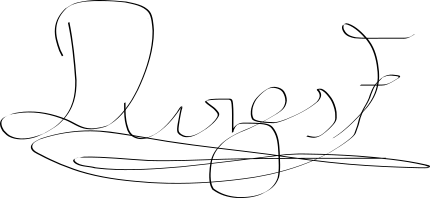
\includegraphics[scale=0.2]{pictures/signature.png}
}


\justifying


\afterpage{%
\vspace{10cm}
\begin{figure*}
    \begin{adjustwidth}{-30mm}{0cm}
        \fbox{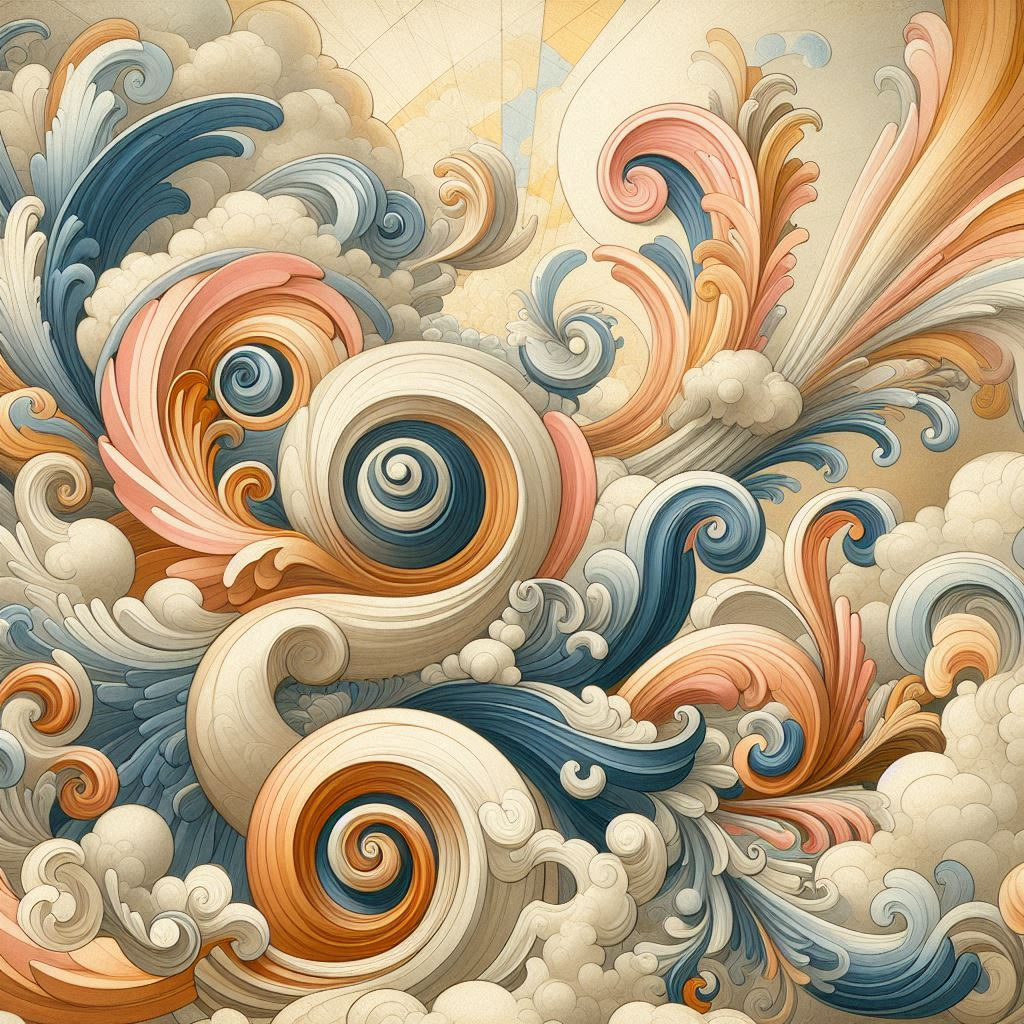
\includegraphics[width=0.9\paperwidth]{pictures/page_garde.jpeg}}
    \end{adjustwidth}
    \caption*{\large Art des Spires et plongée Oniriques, \textit{\small{2025}}}
\end{figure*}
}
\chapter*{Résumé}


Ce travail de recherche s'inscrit dans le cadre du développement de la sécurité face aux attaques par canaux auxiliaires, plus précisément une sous-classe : les attaques temporelles. Cette classe d'attaque nécessite seulement l'usage d'un chronomètre pour être mise en œuvre. Cette facilité d'utilisation a rendu les concepteurs de systèmes sécurisés, notamment de bibliothèques cryptographiques, sensibles à ce type de menace et a permis le développement de contre-mesures. De récents travaux ont malheureusement mis en évidence qu'un code source résistant à ce type d'attaque pouvait redevenir vulnérable si compilé avec un mauvais compilateur. Nous allons présenter un outil permettant d'automatiser la vérification de binaires et ainsi d'attester de la sécurité concrète d'une bibliothèque cryptographique. Pour atteindre cet objectif, nous avons conçu un outil de génération de tests permettant une analyse complète de la bibliothèque étudiée. Nous avons aussi développé un ensemble de protocoles permettant de détailler notre méthodologie et d'effectuer une analyse généralisée à plusieurs architectures et à différents compilateurs.

\bigbreak

\textbf{Mots-clés :} Attaque par canal auxiliaire, temps constant, analyse symbolique, vérification formelle, compilateurs


\cleardoublepage
\tableofcontents*

\newpage\null\thispagestyle{empty}\newpage
\chapter{Tables des illustrations}
\listoffigures
\listoftables
\newpage
\listoflistings


\printindex


\cleardoublepage
\afterpage{%
    \AddToShipoutPictureBG*{%
    \put(2cm,18cm){
        \fbox{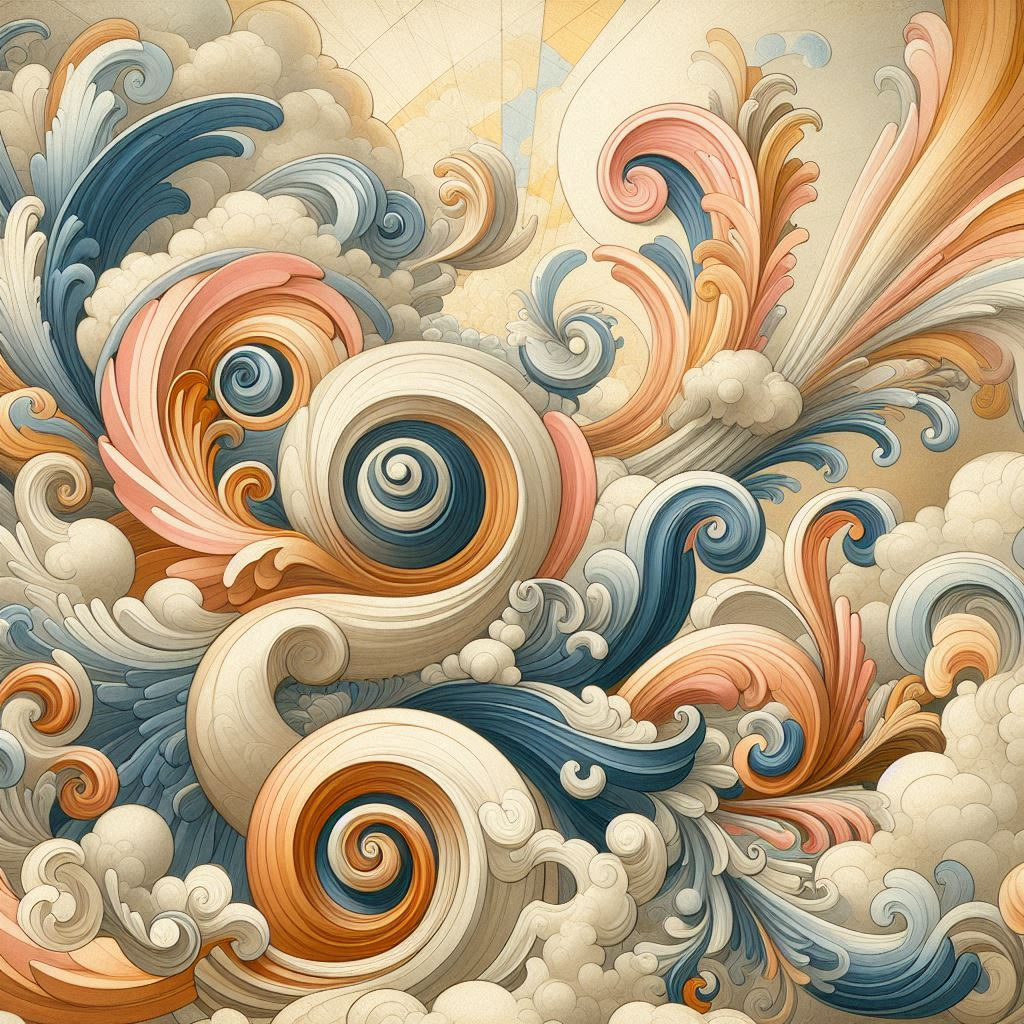
\includegraphics[trim = 0cm 16cm 23cm 0cm, clip, scale = 0.4]{pictures/page_garde.jpeg}}}
    }
    \ClearShipoutPicture%
}
\part{Préambule}

\chapter*{Introduction}
\label{chap:introduction}

Le développement sécurisé est une tâche ardue. Si on porte notre regard vers le langage de programmation C, un guide \cite{progC_guide}\footnote{Développé par Anne Canteaut, chercheuse de l'équipe COSMIQ, récemment entrée à l'Académie des Sciences} porté par l'\indexed{INRIA}\footnote{Institut National de Recherche en Informatique et Automatisme} est complet en 133 pages tandis qu'un guide pour du développement sécurisé\cite{anssi_guideForSecureprogramming} produit par l'\indexed{ANSSI}\footnote{Agence nationale de la Sécurité des Systèmes d'Information} comprends 182 pages. Cette comparaison met en évidence la discipline requise par le développeur pour faire de la programmation sécurisée; en sus des connaissances, pour améliorer son efficacité, en cryptologie, en architecture matérielle et en programmation bas niveau .\medbreak

Malheureusement, malgré ces compétences, des erreurs peuvent être produites puis exploiter pour réaliser des attaques sur ces sytèmes sécurisés. Il existe de nombreuses classe d'attaques, certaines exploitant les défauts de conception (type A) tandis que d'autres utilisent les caractéristiques matériels (type B). Pour limiter ces effets de bords, la pratique de la programmation formelle permet de contraindre le développeur et empêcher l'apparitions de ces erreurs. La production de preuve formelle du code à l'issu de cet exercice permet d'avoir des garanties contres les attaques de type A.

En revanche, pour se défendre d'attaques de type B (ou attaques par canal auxiliaire) dépendantes du matériel support du programme, il est plus difficile d'avoir une méthode miracle. Actuellement, la solution la plus courante est d'identifier les attaques existantes pour ajouter les contre-mesures adéquates permettant d'avoir un système sécurisé. Une sous-classe d'attaque continue malgré tout de résister à cette méthode : les attaques temporelles.\medbreak

Découverte par Paul Kocher en 1996 \cite{crypto-1996-1469}, il les décrit comme <<\textit{une mesure précise du temps requis par des opérations sur les clées secrètes, permettrait à un attaquant de casser le cryptosystème}>>. Face à cette menace, l'enjeu d'avoir un code \textit{\indexed{achrognostique}}\footnote{Néologisme de Thomas Pornin dans son article \textit{Constant-Time Code: The Pessimist Case} \cite{constantTimePornin} pour désigner un code sans connaissance de temps} vient se rajouter aux pratiques de programmations sécurisées. Et pourtant, si contre les attaques de type A on arrive à concevoir des preuves mathématiques de sécurité associées à nos systèmes sécurisés, les garanties contre les attaques de type B sont plus faible ou inexistente.\medbreak

En 2024, les travaux de \citeauthor{schneider2024breakingbadcompilersbreak} \cite{schneider2024breakingbadcompilersbreak} prouvent qu'un usage inadapté de compilateur sur un système sécurisé introdui des failles exploitables. Ces résultats, observables partiellement avec des travaux antérieurs (par exemple \cite{binsecRel2019}), montrent qu'un usage inadéquat d'options fournies au compilateur optimise un code prouvé sécurisé et retire les protections indiquées par le développeur. Cela nous amène à plusieurs questions de recherche (QR) que nous tenterons de répondre à travers ce document.
\begin{enumerate}
    \item[\textbf{QR1}] Est-il possible de détecter les failles qui permettent une attaque temporelles ?
    \item[\textbf{QR2}] Est-il possible d'automatiser la détection de ces failles ?
    \item[\textbf{QR3}] Est-il possible d'étendre ce mécanisme entre différentes architectures ?
\end{enumerate}

Les réponses à ces questions permettraient de développer des systèmes sécurisés, communs entre différents supports et d'avoir des garanties de sécurité.

\begin{Acorriger}{Fin d'introduction - à finir}
    Dans la première section nous reviendrons sur les attaques temporelles, leurs impacts et comment s'en protéger. Puis, Dans la deuxième section nous présenterons les outils disponibles à l'analyse et pour la détection de failles. Nous continuerons, dans la troisième section, avec la présentation de nos contributions. \textit{Enfin, dans la quatrième section nous présenterons les mécanismes présent au plus bas niveau de l'informatique pour se protéger des attaques temporelles.}\medbreak
    Ce travail a été réalisé au sein du centre INRIA de Paris dans le cadre du projet \textit{Everest} concernant la mise au point de Hacl*.
    
\end{Acorriger}

\addcontentsline{toc}{chapter}{Introduction}
\input{chapters/préambule.tex}
\addcontentsline{toc}{chapter}{Préambule}

\mainmatter%%%%%%%%%%%%%%%%%%%%%%%%%%%%%%%%%%%%%%%%%%%%%%%%%%%%%%%%%%%%%
\afterpage{%
    \AddToShipoutPictureBG*{%
    \put(0.25\paperwidth,4cm){
        \fbox{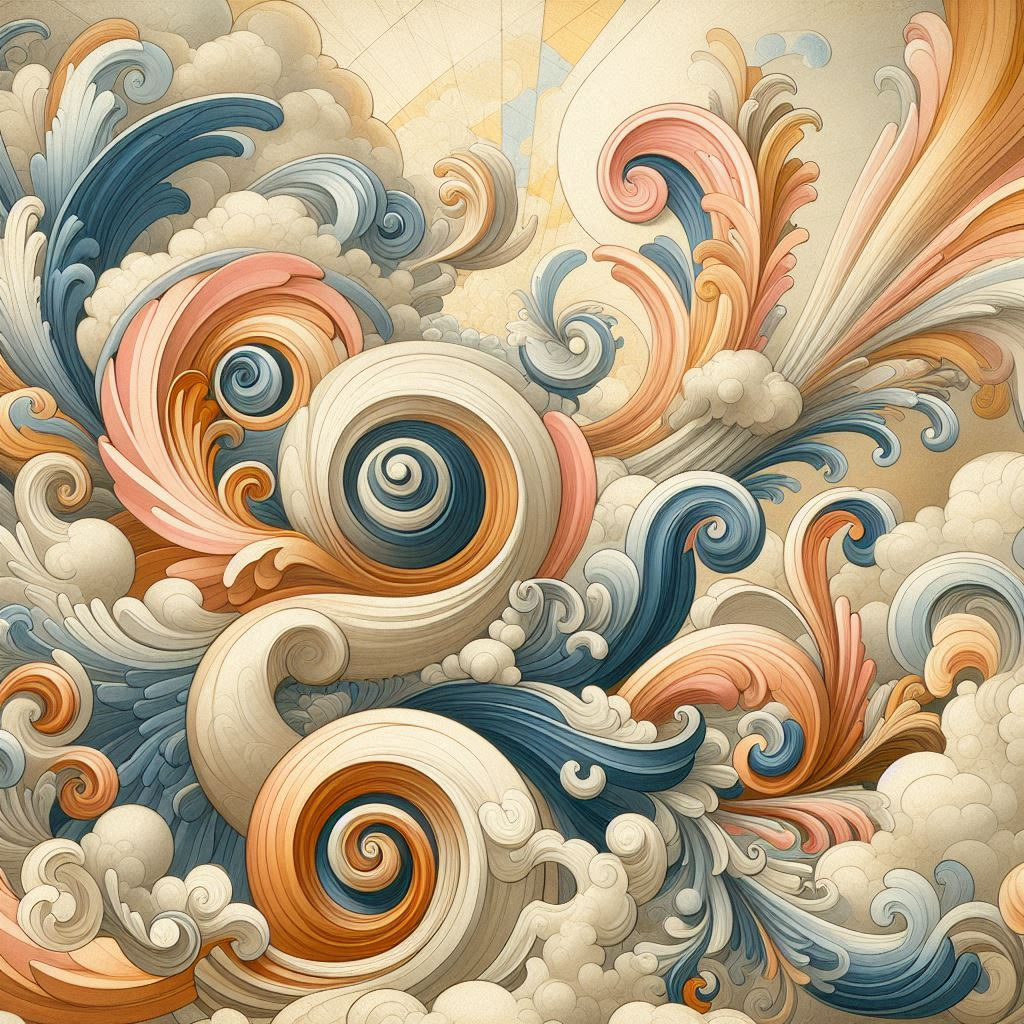
\includegraphics[trim = 16cm 0cm 0cm 23cm, clip, scale = 0.5]{pictures/page_garde.jpeg}}}
    }
    \ClearShipoutPicture%
}
\part{\textit{Constant time} : implémentation et vérification}

\chapter{Présentation, enjeux et attaques}
\label{chap:constantTimePresentation}


Ce premier chapitre a pour but de présenter les enjeux de la sécurité informatique face aux attaques par canal auxiliaire et d'introduire les attaques temporelles. Nous distinguerons les attaques par canal auxiliaire en deux catégories, montrant ainsi la diversité et les potentiels dangers pour un système sécurisé ignorant de cette menace.



\section{L'exécution du code est observable...}

L'Informatique repose sur deux fondations que l'on tend à distinguer dans l'enseignement : le matériel et le logiciel. Pourtant, si on gardait séparé ces deux domaines, on aurait des tas de piles de métal et de plastiques ou des bibliothèques de livres plein d'idées intéressantes. Au contraire, combiner les les deux parties permet de réaliser des prouesses technologoqies et scientifiques. Ainsi, lorsque l'on conçoit un système sécurisé, il faut prendre en compte ces deux composantes. Or pour implémenter un système sécurisé, il ne faut pas seulement un logiciel sécurisé, il est aussi important que le matériel le soit. Oublier comment fonctionne un support informatique, c'est oublier que programmer se résume à manipuler de l'électricité.\medbreak

Les attaques par canal auxiliaires consistent à exploiter les caractéristiques matériels du support pour gagner en connaissances sur le programme ciblé. Puis exploiter ces connaissances pour acquérir d'avantages d'informations privées : identifiants, clés secrètes, messages personnels. On leurs attribue le terme "canal auxiliaire" car il ne s'agit pas d'essayer de pousser dans ses limites un logiciel ou vérifier que tous les cas particulier sont gérés à travers le canal conçus par le développeur (une interface graphique souvent) mais plutôt de se positionner hors du cadre. Voici quelques travaux présentant une attaque par canal auxiliaire et surtout le canal exploité:
\begin{itemize}
    \item[\cite{DPA_Attack}] Consommation d'énergie 
    \item[\cite{Branch_Attack}] Prédiction de branchement 
    \item[\cite{Thermal_Attack}] Variation de température
    \item[\cite{DRAM_Attack}] Accès à la mémoire DRAM
\end{itemize}\medbreak

Le point commun de ces attaques est la nécéssité d'avoir un point de contact avec la cible. Il faut que l'attaquant puisse récupérer le matériel informatique ou le programme qu'il souhaite attaquer pour ensuite poser des sondes/capteurs enfin d'accumuler de la connaissance et monter son exploitation.\bigbreak


Une autre technique d'attaque consiste à venir introduire une erreur dans le déroulement normal d'un programme. Il s'agit d'une attaque par injection de faute. Originellement \cite{faultOverview} les fautes étaient "naturelles" : un défaut dans le code, un problème avec la transcription vers du code machine, un défaut d'un composant dans le système ou un interférence. Ces interférence sont causées par une irrégularité de l'alimentation électrique, des radiations életromagnétique, une perturbation environnementale \etc\dots
En 2004, \citeauthor{Fault_Attacks} dans leur article \citetitle{Fault_Attacks} \cite{Fault_Attacks} effectuent un tour d'horizon des techniques, montrant l'efficacité de cette méthode sur \indexed{RSA}\footnote{Chiffrement asymétrique par clés secrète du nom de ces auteurs. Standardisé en 1983.}, \indexed{NVM}\footnote{Non Volatile Memory ou mémoire non volatile est un composant informatique qui conservent son contenu en l'absence d'électricité.}, \indexed{DES}\footnote{Algorythme de chiffrement symétrique par bloc. Standardisé en 1977}, \indexed{EEPROM}\footnote{Electrically-Erasable Programmable Read-Only Memory ou mémoire morte effaçable électriquement et programmable.}, \indexed{JVM}\footnote{Machine virtuelle qui exécute des programmes compilés en bytecode Java.}. On y retrouve enfin une liste de contre-mesures et de méthodes de protections contre ces attaques.\medbreak

Ainsi, donner un accès physique à un inconnu est une porte d'entrée pour un attaquant. Pourtant, penser que l'accés physique au support est une condition nécessaire et suffisante pour réaliser une attaque par canal auxiliaire est une erreur.

\section{...à distance}

En effet, il est possible de réaliser des attaques à distance en exploitant d'autres failles de sécurité d'un programme ou d'autres caractéristiques matériels. L'attaque présentée par \citeauthor{LLC_attack} dans \citetitle{LLC_attack} \cite{LLC_attack} repose sur la conception des services clouds où les machines virtuelles accèdent au même matériel. Tandis que la virtualisation crée l'illuson de compartimentation entre les sessions, en réalité, les adresses mémoires pointent vers une ressource physique partagée. Ainsi, l'exploitation du cache du dernier niveau (LLC) permet à un co-hôte de récupérer les clés secrètes d'un autre utilisateur. L'attaquant rempli le cache, puis mesure les temps d'accés vers ces registres. Si des modifications apparaissent dans ces temps, cela signifie que la victime a accédé à ces registres. En répétant cette opération, l'attaquant peut reconstruire les clés secrètes de la victime.\medbreak


D'autres attaques distantes comme celle de \citeauthor{LLC_attack} existent \cite{cryptoeprint:2016/224,Moghimi_2017,vanbulck2018nemesis}, mais on observe rapidement que ces techniques emploient aussi la méthode de chronométrage. En effet, si on cible un algorithme et que l'on mesure son temps d'exécution. Si en fournissant différentes entrées (que l'on considère secrètes) des variations sont observées entre les mesures, alors cela signifie que l'algorithme présente une dépendance à ces entrées. Généralement une sous-fonction de cet algorithme est responsable de ces variations. Cette classe d'attaque est appelée <<\textit{attaque temporelle}>>\footnote{Le terme générique dans la recherche scientifique est <<\textit{time attack}>>. Une traduction plus précise serait <<\textit{attaque par chronométrage}>>. on choisit ici d'utiliser le terme <<\textit{attaque temporelle}>> car il est moins lourd et renvoie directement vers la faille exploitée plutôt que sur la méthode employée.}.\medbreak

Le lien entre temps et exécution de code est connu depuis le début de l'informatique. Le temps est le marqueur de performance, d'efficacité d'un programme. En revanche, l'idée d'exploiter cet indice pour réaliser une attaque est arrivée plus tardivement. \citeauthor{crypto-1996-1469} nous présente le premier, en 1996, comment monter une attaque en utilisant ce canal.\medbreak

Ce lien entre temps et exécution est connu, pourtant la mesure de l'ampleur de la fuite d'information transmise par ce canal n'est pas triviale; ni à son époque, ni à celle-ci.

\begin{listing}[!ht]
    \caption{Exemple de code vulnérable à une attaque temporelle}
    \label{lst:timing_attack_example}
    \begin{minted}[frame=lines,framesep=2mm,baselinestretch=1.2,fontsize=\footnotesize,linenos, gobble=6]{C}
        bool check_pwd(msg, pwd){
        if (msg.length != pwd.length){
            return False
        }
        for(int i = 0; i < msg.length; i++){
            if(msg[i] != pwd[i]){
            return False
            }
        }
        return True
        }
    \end{minted}
\end{listing}
                
Si nous prenons le code présenté par le code \ref{lst:timing_attack_example}, on peut observer que la fonction \texttt{check\_pwd} compare deux chaînes de caractères. Si elles sont de même longueur, elle les compare caractère par caractère. Si elles sont de longueurs différentes, la fonction retourne immédiatement \texttt{False}. Ainsi, si l'on fournit un mot de passe de longueur différente, le temps d'exécution sera constant et court. En revanche, si l'on fournit un mot de passe de même longueur, le temps d'exécution dépendra du nombre de caractères identiques entre les deux chaînes. En effet, la fonction s'arrêtera dès qu'un caractère différent est trouvé. Ainsi, en mesurant le temps d'exécution pour différents mots de passe, un attaquant peut déduire des informations sur le mot de passe correct.\medbreak

On peut synthétiser les éxécutions de la fonction \texttt{check\_pwd} en un graphe comme celui présenté par la figure \ref{fig:timing_attack_example}. Chaque interruption de la fonction peut être observée et mesurée, permettant ainsi de régénérer le mot de passe. Bien sûr la connaissance du protocole cible est requise ou alors il faut réaliser un travail de rétro-ingénierie pour calibrer l'attaque.\medbreak

\begin{figure}[!ht]
    \caption{Suivi du temps d'exécution pour différents mots de passe}
    \label{fig:timing_attack_example}
    \center
    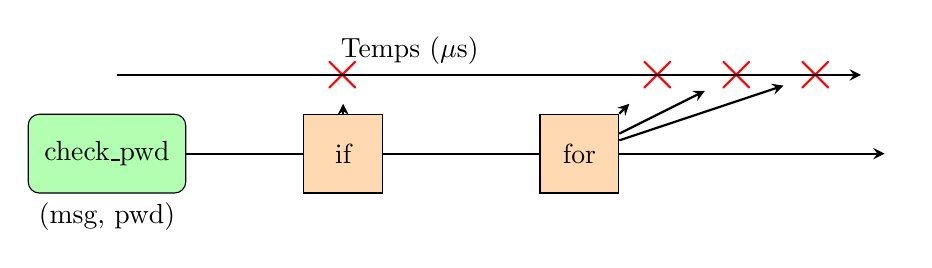
\begin{tikzpicture}[auto]

    % Styles
    \tikzstyle{startstop} = [rectangle, rounded corners, minimum width=2cm, minimum height=1cm, text centered, draw=black, fill=green!30]
    \tikzstyle{process} = [rectangle, minimum width=1cm, minimum height=1cm, text centered, draw=black, fill=orange!30]
    \tikzstyle{arrow} = [thick,->,>=stealth]
    \tikzstyle{arrowred} = [thick,->,>=stealth, draw=red]
    
    % Noeuds
    \node (start) [startstop] {check\_pwd};
    \node (valid) [right of=start, xshift=9cm, green] {\huge{$\checkmark$}};
    \draw [arrow] (start) -- (valid);
    
    \node (inputs) [below of = start, yshift=0.2cm] {(msg, pwd)};
    \node (if) [process] [right of=start, xshift=2cm] {if};
    \node (not) [above of=if, red] {\huge{$\times$}};
    \node (for) [process] [right of=if,, xshift=2cm] {for};
    \node (for1) [above of=for,xshift=1cm, red] {\huge{$\times$}};
    \node (for2) [right of=for1, red] {\huge{$\times$}};
    \node (for3) [right of=for2, red] {\huge{$\times$}};

    \draw [arrow] (if) -- (not);
    \draw [arrow] (for) -- (for1);
    \draw [arrow] (for) -- (for2);
    \draw [arrow] (for) -- (for3);

    \node (t) [above of=start] {};
    \node (a) [above of=valid, xshift=-0.3cm] {};
    \draw [arrow] (t) -- node[above left] {Temps ($\mu$s)} (a.west);
    
    \end{tikzpicture}
\end{figure}

Cette méthode est plus efficace qu'une attaque par force brute. En effet, si l'on suppose que le mot de passe est de 8 caractères de l'alphabet latin. On a alors  256 possibilités par caractère, pour un total de $256^8 = 2^{64}$ possibilités. En revanche, si l'on utilise la méthode de l'attaque temporelle, on peut réduire le nombre de possibilités à $8 + 8 \times 256 = 2056$ possibilités. En effet, on cherche dans un premier temps à identifier la longueur du mot de passe, puis on identifie charactère après charactère pour trouver le bon secret. Avec des temps d'exécution court on est dans les cas de figure d'échec, tandis qu'avec un allongement du temps d'exécution on sait que l'on est sur la bonne piste.\medbreak

Les attaques temporelles présentent la particularité d'être générique. Tandis que les attaques décrites précédemment nécessite des conditions d'accés ou d'initialisation plus importante, cette classse d'attaque présente l'avantage d'être réalisable sur tous les types de systèmes, et notamment les systèmes accessible par internet. La connaissance de cette menace est donc primordiale pour l'implémentation et la mise en service de produit sur internet.\medbreak

Par la suite du document, le terme "fuite" sera utilisé pour désigner un extrait du programme qui peut être exploité pour réaliser une attaque temporelle. Si on reprend le code \ref{lst:timing_attack_example}, les branchement conditionnels ligne [4,6] sont des fuites d'informations. C'est grâce à ces instructions que l'attaque décrite précedemment est réalisable.\medbreak

\raggedbottom
\textit{Nous allons maintenant nous intéresser aux moyens et méthodes à notre disposition pour se protéger contre les attaques temporelles.}
\chapter{Protection}
\label{chap:constantTimeSolution}

Ce deuxième chapitre montre les innovations nécessaires pour se protéger des attaques temporelles. On y découvre les bonnes pratiques de programmation, les premiers outils automatique de vérification de code ainsi que les limitations auquelles est confronté le développeur qui souhaite être résistant à ces attaques.


\section{Bonne pratique et usages}

Face à la menace des attaques temporelles, quelles solutions peuvent être mises en place pour protéger nos systèmes informatiques ? Cette attaque a besoin d'un accès au système et d'un chronomètre. Comme on est dans un contexte de systèmes accessibles par internet, altérer ou retirer l'accès signifie perdre en qualité ou supprimer le service proposé. Il faut donc que notre approche cible plutôt l'utilisation du chronomètre.

Il faut donc programmer de tel sorte que sur toutes les entrées possibles de notre système informatique aucune variation de temps ne peut être observée entre les exécutions.
Trois méthodes existent pour pallier à ce problème.\medbreak

\subsection*{Programmation en temps constant}
La programmation en temps constant ou <<\textit{Constant-Time Programming}>>, est une pratique de programmation qui vise à résoudre exactement ce problème. Directement lié à la compléxité algorithmique, cette pratique modifie et adapte les algorithmes pour que toutes les opérations effectuées aient un temps d'exécution identique.

\citeauthor{BearSSL} \cite{BearSSL} présente tous les éléments à adapter pour configurer un code respectant la politique de programmation en temps constant. Si les opérations élémentaires respectent "naturellement" cette politique; les \textbf{accès mémoires}, les \textbf{sauts conditionnels}, les \textbf{sopérations de décalages/rotations} et les \textbf{divisions/multiplications} sont les opérations à adapter en fonction de la plateforme cible. Les descriptions rapportées ci-dessous sont issues de \cite{BearSSL}.\smallbreak

\begin{CitationBox}{Accès mémoire}
  Un chargement depuis la mémoire d'une information est une source de variation. On a vs précedemment \cite{LLC_attack,DRAM_Attack} que l'usage d'un cache mémoire est un canal d'accès pour réaliser une attaque. En effet, l'utilisation d'un cache permet de distinguer les appels entre les données déjà mises en mémoire ou pas. De plus, les changements de valeur dans celui-ci peuvent aussi être observé après exécution.
\end{CitationBox}
\vspace{0.1cm}
\begin{CitationBox}{Décalage et rotation}
  Ces opérations binaires sont ou ne sont pas en temps constant en fonction des CPU sur lequel le code est exécuté. Certains ont un "barrel shifter" qui permet d'effectuer directement les instructions correspondantes. Cela impacte directement les algorithmes dépendant de décalages logiques comme le chiffrement RC5.
\end{CitationBox}
\vspace{0.1cm}
\begin{CitationBox}{Saut conditionnel}
  Les saut conditionnels sont des instructions qui, comme pour les accès mémoires, demandent de charger les adresses des instructions suivantes. Or, comme un compilateur tend à précharger les instructions suivantes, il va charger les deux côtés du saut conditionnel puis defausser la branche inutile; ce qui entraîne un léger alentissement. En revanche, il est important de noter que si le branchement est indépendant d'une variable secrète, il n'est pas nécessaire de le modifier. Par exemple si j'ai un compteur et que mon programme doit terminer après un certain nombre d'itérations, aucune fuite ne sera observée.
\end{CitationBox}
\vspace{0.1cm}
\begin{CitationBox}{Division}
  Certaines architectures ont des instructions de divisions spécifiques qui permettent d'accélérer le calcul, les autres emploient des sous-programmes dédiées souvent optimisés en opération de masquage et de décalage. La norme C entraîne elle aussi de la confusion car elle impose $(-1)/2 = 0$; il faut donc être familier avec les spécificités du processeur pour affiner l'usage de cette opération.
\end{CitationBox}
\vspace{0.1cm}
\begin{CitationBox}{Multiplication}
  Enfin, la multiplication, elle aussi dépendante des variable d'entrées, présente une fuite d'information importante. Mais les CPU les plus récents (rédigé en 2016) ont implémenté cette opération en temps constant. Cela suit l'évolution des compilateurs et des processeurs qui tendent à accélérer les opérations et réduire le nombre d'instruction total.
\end{CitationBox}
\vspace{0.1cm}

En reprennant ces règles, on peut modifier notre exemple de code \ref{lst:timing_attack_example} et appliquer des modifications sur lignes que l'on a déjà ciblées comme fuites d'informations. Les modifications sont libre au choix du concepteur. Voici une correction qui peut être réalisée :

\begin{listing}[!htb]
    \caption{Exemple de correction pour rendre un code résistant aux attaques temporelles}
    \label{lst:timing_attack_CT_example}
    \begin{minted}[frame=lines,framesep=2mm,baselinestretch=1.2,fontsize=\footnotesize,linenos, gobble=6]{C}
        bool check_pwd(msg,pwd) {
          // Hachage
            char msg_hash[SHA256_DIGEST_LENGTH]; sha256_hash_string(msg, msg_hash);
            char pwd_hash[SHA256_DIGEST_LENGTH]; sha256_hash_string(pwd, pwd_hash);

            // Comparaison
            bool equal = true;
            for (int i = 0; i < SHA256_DIGEST_LENGTH; i++) {
                if (msg_hash[i] != pwd_hash[i]) {
                    equal = equal && false;
                } else {
                    equal = equal || false;
                }
            }
            return equal;
        }
    \end{minted}
\end{listing}

On voit que le premier branchement a été remplacé par un hachage des paramètres d'entrées. Cette opération est considérée ici en temps constant mais peut ne pas l'être. Il faut être vigilant sur toutes les briques d'algorithme que l'on souhaite utiliser. Enfin, le second branchement conditionnel est purement supprimé, le parcours des tableaux se fait entièrement.\bigbreak

Avec cette modification, on a un code \ref{lst:timing_attack_CT_example} qui ne présente plus de fuite de données. Pourtant, on peut avoir un doute sur l'usage de la fonction "\textit{sha256\_hash\_string}". Si cette fonction n'est pas elle même implémentée selon la politique temps constant, on a alors introduis une nouvelle surface de fuite d'informations. Il faut vérifier notre code pour supprimer ce doute.\medbreak

\subsection*{Outils de garanties}

Plusieurs outils existent est peuvent être utilisés tous au long du processus de développement d'un système sécurisé. Cela peut être durant la phase de conception du code source, au moment de la compilation ou encore en vérification de la compilation.\smallbreak


Une solution légère est de ce servir du système libre <<\textbf{Compiler Explorer}\footnote{\url{https://godbolt.org/}}>>. Avec à disposition un éditeur de texte, il est possible de voir comment sera généré le code assembleur. En reprenant une partie du code \ref{fig:timing_attack_example}, on peut voir sur la figure \ref{img:godbolt_example} que le choix du compilateur, ici sa version, introduit une légère modification. Ce changement n'est pas perceptible sans observation directe, il se perçoit directement grâce à la petite taille du code observé.

\begin{figure}[!h]
  \begin{adjustwidth}{-2.5cm}{-2cm}
    \centering
    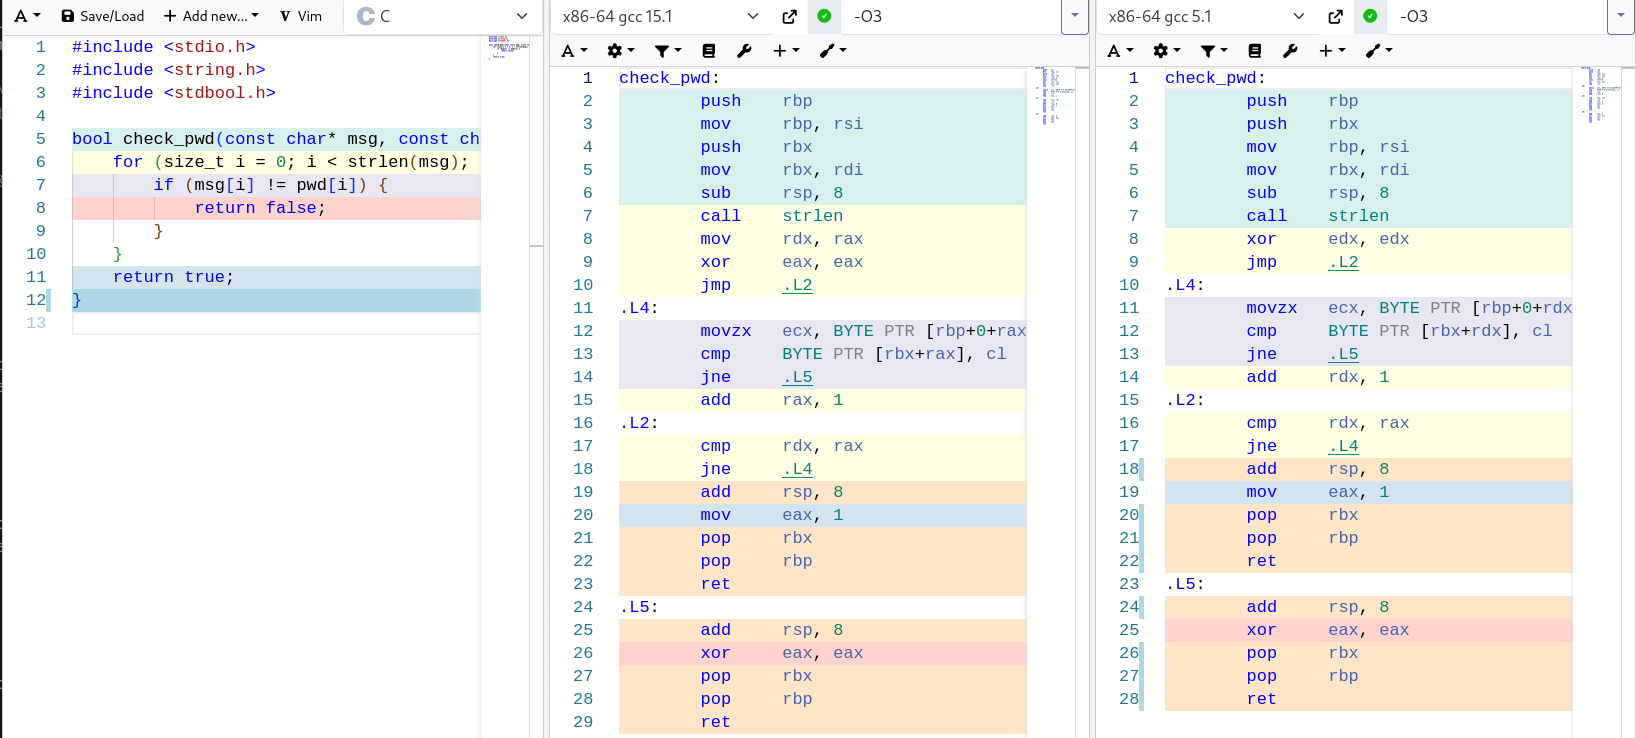
\includegraphics[trim = 1mm 0mm 0mm 0mm, clip,width=0.9\paperwidth]{pictures/godbolt_example.png}
    \caption{Capture d'écran de comparaison de code assembleur x86\_64 entre \texttt{GCC 15.1} et \texttt{GCC 5.1}}
    \label{img:godbolt_example}
  \end{adjustwidth}
\end{figure}

Si l'on souhaite faire une analyse à l'échelle d'un projet, ce parcours à la main des fonctions ou de morceaux de fonctions est réellement fastidieux. Il faut mieux déléguer ce travail à un outil conçus pour vérifier la présence de fuite.\smallbreak

Plusieurs articles références l'ensemble des outils existant \cite{notThatHardCT, GeimerEvaluationsSideChannel} pour réaliser ce travail. Le tableau \ref{tab:tools_ct} de \citeauthor{notThatHardCT} liste 24 outils en libre accès conçus pour détecter des failles par canal auxiliaire.

Ils sont listés alphabétiquement et sont précisé le type de fichier analysé (\textit{Cible}), la méthode d'analyse réalisée (\textit{Techn.}) et les garanties attendues de ces analyses (\textit{Garanties}). On reviendra plus en avant avec ces détails de méthodes et de fonctionnement dans le chapitre \ref{chap:automateVerifOutils}.\medbreak

\begin{table}[!ht]
  \caption{Liste d'outils de vérification, source \cite{notThatHardCT} }
  \label{tab:tools_ct}
  \scriptsize{
  Cible : [C, Java] = Code source, Binaire = Binaire, DSL = Surcouche de langage, Trace = Trace d'exécution, WASM = Assembleur web.\\
  Techn. : Formel = Programmation formelle, [Symbolique, Dynamique, Statistique] = type d'analyse. \\
  Garanties (\textit{Sécurité face aux attaques temporelles}) : $\bullet$ = Analyse correct, $\blacktriangle$ = Correct mais avec des limitations, $\circ$ = Aucune garantie, $\bigstar$ = Vérification d'autres propriétés.
  }
  \normalsize
  \begin{center}
    \begin{tabular}{lccc}
    \hlineB{2}
    \textbf{Outil} & \textbf{Cible} & \textbf{Techn.} & \textbf{Garanties} \\
    \rowcolor{lightgray}
    ABPV13 \cite{ABPV13} & C & Formel & $\bullet$ \\
    Binsec/Rel \cite{binsecRel2019} & Binaire & Symbolique & $\blacktriangle$ \\
    \rowcolor{lightgray}
    Blazer \cite{Blazer} & Java & Formel & $\bullet$ \\
    BPT17 \cite{BPT17} & C & Symbolique & $\blacktriangle$ \\
    \rowcolor{lightgray}
    CacheAudit \cite{CacheAudit} & Binaire & Formel & $\bigstar$ \\
    CacheD \cite{CacheD} & Trace & Symbolique & $\circ $ \\
    \rowcolor{lightgray}
    COCO-CHANNEL \cite{COCOCHANNEL} & Java & Symbolique & $\bullet$ \\
    ctgrind \cite{ctgrind} & Binaire & Dynamique & $\blacktriangle$ \\
    \rowcolor{lightgray}
    ct-fuzz \cite{ctfuzz} & LLVM & Dynamique & $\circ$ \\
    ct-verif \cite{ctverif} & LLVM & Formel & $\bullet$ \\
    \rowcolor{lightgray}
    CT-WASM \cite{CTWASM} & WASM & Formel & $\bullet$ \\
    DATA \cite{DATA1,DATA2} & Binaire & Dynamique & $\blacktriangle$ \\
    \rowcolor{lightgray}
    dudect \cite{dudect} & Binaire & Statistique & $\circ $ \\
    FaCT \cite{FaCT} & DSL & Formel & $\bullet$ \\
    \rowcolor{lightgray}
    FlowTracker \cite{FlowTracker} & LLVM & Formel & $\bullet$ \\
    haybale-pitchfork \cite{haybale-pitchfork} & LLVM & Symbolique & $\blacktriangle$ \\
    \rowcolor{lightgray}
    KMO12 \cite{KMO12} & Binaire & Formel & $\bigstar$ \\
    MemSan \cite{MemSan} & LLVM & Dynamique & $\blacktriangle$ \\
    \rowcolor{lightgray}
    MicroWalk \cite{MicroWalk} & Binaire & Dynamique & $\blacktriangle$ \\
    SC-Eliminator \cite{SCEliminator} & LLVM & Formel & $\bullet$ \\
    \rowcolor{lightgray}
    SideTrail \cite{SideTrail} & LLVM & Formel & $\bigstar$ \\
    Themis \cite{Themis} & Java & Formel & $\bullet$ \\
    \rowcolor{lightgray}
    timecop \cite{timecop} & Binaire & Dynamique & $\blacktriangle$ \\
    VirtualCert \cite{VirtualCert} & x86 & Formel & $\bullet$ \\
    \hlineB{2}
    \end{tabular}
  \end{center}
\end{table}

\newpage
Une dernière solution serait d'utiliser un compilateur spécialisé qui produit un code assembleur sans fuite \cite{Borrello_2021, Raccoon} ou d'utiliser un compilateur formel comme \textit{CompCert} \cite{CompCert}. Cette solution rencontre en pratique de nombreux problèmes que l'on se garde pour la section \ref{sect:limitations} \nameref{sect:limitations}.

\subsection*{Écriture en code assembleur}

Enfin, la dernière méthode pour obtenir un code sécurisé et sans fuite c'est de programmer directment en assembleur. De cette manière, on a un contrôle total sur le flot d'exécution de notre programme, on peut ainsi insérer des optimisations qu'un compilateur pourrait ignorer. Écrire en assembleur requiert de connaître la plupart des opérandes disponibles pour l'architecture que l'on cible et les modèles des composants présents sur le support. Cela nous amène directement aux limitations induites par cette solution.

\section{Limitations}
\label{sect:limitations}

Écrire en assembleur c'est écrire spécifiquement pour une architecture de processeur. Il faut connaître les instructions adéquates, les potentielles optimisations qui existent sans parler de la synthaxe particulère qui rend son développement plus lent. Travailler en assembleur c'est limiter la portabilité du code proposé. Or l'objectif derrière le développement d'une librairie sécurisée est de pouvoir être employée par le plus de configurations possibles pour se protéger d'attaques.\smallbreak

Face à cette situation, on choisit donc d'utiliser un compilateur spécialisé (\cite{Borrello_2021, Raccoon}). Et à nouveau on se retrouve limité parce que ces compilateurs ne supportent pas l'ensemble du jeu d'instruction d'une architecture, ont besoin d'instructions supplémentaires (des annotations de code) pour réaliser la compilation, n'implémente pas les optimisations qui apparaissent sur les processeurs les plus récents ou encore ne sont adaptés qu'à un seul langage de programmation.\smallbreak

À nouveau, on se retrouve donc à utiliser les compilateurs communs \texttt{GCC} et \texttt{LLVM} pour notre solution sécurisée. On se doit donc de programmer en respectant la politique temps constant. Et si cette pratique semble faire ses preuves, on peut lire dans la présentation de l'outil d'analyse Binsec \citetitle{binsecRel2019} : 
\begin{CitationBox}{Conclusion - \cite{binsecRel2019}}
Nous avons découvert que \texttt{gcc -O0} et des optimisations de \texttt{clang} introduisent des infractions à la politique temps constant indétectées par les outils antérieurs
\end{CitationBox}\smallbreak

Cette annonce a ensuite été prise en compte par \citeauthor{schneider2024breakingbadcompilersbreak} qui a mené une enquête sur les bibliothèques cryptographiques sécurisées et résistantes aux attaques temporelles : \cite{schneider2024breakingbadcompilersbreak}. La conclusion principale est que les compilateurs modernes sont devenus assez performants pour voir à travers les astuces employées et qu'une mauvaise utilisation d'optimisation implique l'introduction de faille de sécurité. \smallbreak

Voici un exemple communiqué par \citeauthor{schneider2024breakingbadcompilersbreak} auprès des chercheurs de Hacl*. On peut voir deux fonctions dans le code \ref{lst:Hacl_masking}, <<\textit{cmovznz4}>> et <<\textit{FStar\_UInt64\_eq\_mask}>>. La première appelle la seconde pour générer un masque qui sera ensuite appliqué au entrée de <<\textit{cmovznz4}>>. On a ici une fonction qui agit comme un branchement conditionnel. Si \texttt{cin} vaut 1, alors $r = x$ sinon $r = y$.

\begin{listing}[!ht]
    \caption{Fonction de masquage issu de \textit{Hacl*}}
    \label{lst:Hacl_masking}
    \begin{minted}[frame=lines,framesep=2mm,baselinestretch=1.2,fontsize=\footnotesize,linenos]{C}
#include <stdint.h>

static inline uint64_t FStar_UInt64_eq_mask(uint64_t a, uint64_t b)
{
  uint64_t x = a ^ b;
  uint64_t minus_x = ~x + (uint64_t)1U;
  uint64_t x_or_minus_x = x | minus_x;
  uint64_t xnx = x_or_minus_x >> (uint32_t)63U;
  return xnx - (uint64_t)1U;
}

void cmovznz4(uint64_t cin, uint64_t *x, uint64_t *y, uint64_t *r)
{
  uint64_t mask = ~FStar_UInt64_eq_mask(cin, (uint64_t)0U);
  uint64_t r0 = (y[0U] & mask) | (x[0U] & ~mask);
  uint64_t r1 = (y[1U] & mask) | (x[1U] & ~mask);
  uint64_t r2 = (y[2U] & mask) | (x[2U] & ~mask);
  uint64_t r3 = (y[3U] & mask) | (x[3U] & ~mask);
  r[0U] = r0;
  r[1U] = r1;
  r[2U] = r2;
  r[3U] = r3;
}
    \end{minted}
\end{listing}

Avec le compilateur \texttt{RISC-V rv64gc clang 15.0.0}, si on entre les options de compilation \texttt{-O0} ou \texttt{-O1} on peut observer différents résultats. Le plus notable ici est l'apparition de l'instruction \texttt{beqz}, qui est un branchement conditionnel, ainsi que la suppression de la fonction de masquage <<\textit{FStar\_UInt64\_eq\_mask}>>. Les optimisations appelées par l'option \texttt{-O1} identifient le masquage réalisé et modifient le code pour accélérer son exécution. L'optimisation \ref{subcode:O0} suient les instructions précisées par le code source, de cette manière le compilateur réalise une compilation rapide. Au contraire dde l'optimisation \ref{subcode:O1} qui réalise une analyse plus longue du code source, et donc a une compilation plus lente, mais grâce à l'ajout des branchements succesifs (les instructions \texttt{beqz}) permet une exécution plus rapide. Les options de compilations sont rapportées en annexe \ref{tab:compile_option}\footnote{\url{https://gcc.gnu.org/}}.

\begin{figure}[!ht]
    \begin{subfigure}[b]{0.5\textwidth}
        \centering
        \small
        \begin{minted}[frame=single, framesep=2mm, baselinestretch=1.2, fontsize=\footnotesize, linenos]{java}
cmovznz4:
        ...
        li      a1, 0
        call    FStar_UInt64_eq_mask
        not     a0, a0
        sd      a0, -56(s0)
        ld      a0, -40(s0)
        ld      a0, 0(a0)
        ld      a2, -56(s0)
        and     a0, a0, a2
        ld      a1, -32(s0)
        ld      a1, 0(a1)
        not     a2, a2
        and     a1, a1, a2
        or      a0, a0, a1
        sd      a0, -64(s0)
        ...
        ret

FStar_UInt64_eq_mask:
        addi    sp, sp, -64
        sd      ra, 56(sp)
        sd      s0, 48(sp)
        addi    s0, sp, 64
        sd      a0, -24(s0)
        sd      a1, -32(s0)
        ld      a0, -24(s0)
        ld      a1, -32(s0)
        xor     a0, a0, a1
        sd      a0, -40(s0)
        ld      a1, -40(s0)
        li      a0, 0
        sub     a0, a0, a1
        sd      a0, -48(s0)
        ld      a0, -40(s0)
        ld      a1, -48(s0)
        or      a0, a0, a1
        sd      a0, -56(s0)
        ld      a0, -56(s0)
        srli    a0, a0, 63
        sd      a0, -64(s0)
        ld      a0, -64(s0)
        addi    a0, a0, -1
        ld      ra, 56(sp)
        ld      s0, 48(sp)
        addi    sp, sp, 64
        ret
        \end{minted}
        \caption{Option \texttt{-O0}}
        \label{subcode:O0}
    \end{subfigure}%
    ~~
    \begin{subfigure}[b]{0.4\textwidth}
        \centering
        \small
        \begin{minted}[frame=single, framesep=2mm, baselinestretch=1.2, fontsize=\footnotesize, linenos]{java}
cmovznz4:
        mv      a5, a1
        beqz    a0, .LBB0_2
        mv      a5, a2
.LBB0_2:
        beqz    a0, .LBB0_5
        addi    a6, a2, 8
        bnez    a0, .LBB0_6
.LBB0_4:
        addi    a4, a1, 16
        j       .LBB0_7
.LBB0_5:
        addi    a6, a1, 8
        beqz    a0, .LBB0_4
.LBB0_6:
        addi    a4, a2, 16
.LBB0_7:
        ld      a7, 0(a5)
        ld      a5, 0(a6)
        ld      a6, 0(a4)
        beqz    a0, .LBB0_9
        addi    a0, a2, 24
        j       .LBB0_10
.LBB0_9:
        addi    a0, a1, 24
.LBB0_10:
        ld      a0, 0(a0)
        sd      a7, 0(a3)
        sd      a5, 8(a3)
        sd      a6, 16(a3)
        sd      a0, 24(a3)
        ret
        \end{minted}
        \caption{Option \texttt{-O1}}
        \label{subcode:O1}
    \end{subfigure}
    \caption{Comparaison du code \ref{lst:Hacl_masking} en fonction de différentes options de compilation données au compilateur, réalisée avec l'aide de \textit{Compiler Explorer}.}
\end{figure}

\raggedbottom
\textit{Transition}

\chapter{Analyse de programmes et méthodes de vérifications}
\label{chap:automateVerifOutils}

Nous allons étudier les moyens à notre disposition pour réaliser une analyse pertinente et efficace d'un programme résistant aux attaques temporelles.

\section{Modélisation d'une attaque}

En sécurité informatique, la première étape, essentielle avant de développer une solution, c'est de produire un modèle du danger dont l'on souhaite se défendre. On parle parfois de \textit{modèle de fuite}. Cette étape de synthèse et d'abstraction est importante pour identifier les risques encourus par le futur système, souvent en identifiant les points de fuites employés par les attaques déjà publiées. \citeauthor{BewarCTSideChannel} \cite{BewarCTSideChannel} nous donne les trois modèles d'adversaires que nous devons considérer lorsqu'on souhaite se défendre contre les attaques temporelles :

\begin{table}[!ht]
  \caption{Modèles d'adversaires pour les attaques temporelles \cite{BewarCTSideChannel}}
  \label{tab:temporal_attacks}
  \begin{adjustbox}{width=\textwidth}
  \begin{tabularx}{\textwidth}{|L|L|}
    \hline
    \rowcolor{lightgray}
    \multicolumn{1}{|C|}{\textbf{Type d'attaque}} & \multicolumn{1}{C|}{\textbf{Description}} \\ \hline
    Par chronométrage & Observation du temps de calcul. \\ \hline
    Par accès mémoire & Manipulation et observation des états d'un ou des caches mémoires. \\ \hline
    Par récupération de traces & Suivi des appels de fonctions, des accès réussis ou manqués à la mémoire. \\ \hline
  \end{tabularx}
  \end{adjustbox}
\end{table}

Ces types d'attaques forment une base pour la conception de nos modèles d'attaquant. Considérer le mode opératoire <<récupération de traces>> induit un modèle plus fort. Des travaux comme ceux de \citeauthor{twartingCT} \cite{twartingCT} portent directement sur des améliorations matérielles permettant une défense contre ce modèle. Considérer un hypothétique attaquant plus puissant, avec des accès à des ressources supplémentaires, permet de concevoir un système plus sûr. Certains outils comme \cite{ctfuzz,DATA2} ou cette étude \cite{notThatHardCT} exploitent notamment cette mécanique pour attester de la sécurité d'un programme.\medbreak


Puis, avec ces modèles et les contre-mesures connues, nous pouvons constituer un ensemble de règles qui vérifient ces risques. \cite{CTsaferCrypto} résume celles-ci en une liste de trois règles :
\begin{enumerate}
  \item Toute boucle révèle le nombre d'itérations effectuées. 
  \item Tout accès mémoire révèle l'adresse (ou l'indice) accédé.
  \item Toute instruction conditionnelle révèle quelle branche a été prise.
\end{enumerate}

Avec ces règles, il est alors possible de créer un outil qui analyse les programmes à sécuriser. C'est de cette façon que le premier outil existant a été produit : \texttt{ctgrind} (2010).\medbreak

D'autres chercheurs comme \citeauthor{binsecRel2019} \cite{binsecRel2019} s'attellent à la création de modèles formels. Cette méthode demande un travail de formalisation du comportement de programmes binaire et une implémentation plus rigoureuse de leurs outils. Cela permet en retour une évaluation complète et correcte de programmes complexes (\ie primitives cryptographiques asymétriques).

\subsection*{Formalisation de modèle - \cite{binsecRel2019}}

Si nous voulons concevoir un modèle formel, nous pouvons nous appuyer sur l'article \citetitle{formalConstantTime} \cite{formalConstantTime}.\medbreak


Nous commençons par définir un programme. Il s'agit d'une suite d'instructions binaire. Et une instruction est une action sur la mémoire. Cela nous permet de définir notre programme comme une suite de configurations $(l,r,m)$; $l$ la ligne d'instruction, $r$ le dictionnaire de registre et $m$ la mémoire. La configuration initiale est définie par $c_0 \triangleq (l_0,r_0,m_0)$ où $l_0$ est l'adresse de l'instruction d'entrée du programme, $r_0$ un dictionnaire de registres vide et $m_0$ une mémoire vide.\smallbreak

Ainsi, avec cette modélisation, une instruction est un changement appliqué à notre configuration. Ce changement peut être représenté par $ c_0 \underset{t}{\to} c_1 $, $c_0$ et $c_1$ deux configurations successives, $\to$ la transition entre les deux et $t$ une fuite émise par cette transition. Notons que certaines instructions ne produisent pas de fuites.\smallbreak

Une fois ce préambule installé nous définissons formellement le comportement de nos instructions. Regardons par exemple comment se formalise un chargement :

\begin{figure}[!ht]
  \caption{Instruction \texttt{chargement}}
  \label{fig:instr_load}
  \centering
  
    % version avec \scalebox
    \scalebox{1.8}{% agrandir à 150%
    $\smash{\scalebox{0.5556}{\textsc{LOAD}}}\quad
    \frac{(l,r,m)\; e \vdash_t \text{bv}}
         {(l,r,m)\; @ \; e \vdash_{t.[\text{bv}]} m \;\text{bv}}$
    }
\end{figure}

Ici, l'évaluation de l'expression \texttt{e} sur une configuration $(l,r,m)$ produit une fuite de la valeur $bv$. En haut nous retrouvons la notation de l'opération effectuée et au-dessous la formalisation de la fuite : $t \cdot [bv]$ signifie que la valeur $bv$ s'ajoute à la liste des fuites. Ce second exemple \ref{fig:instr_branchement} présente une opération de branchement en fonction de $e$ vers les instructions $l_1$ et $l_2$. Nous voyons que la valeur est différente de zéro, ce qui nous produit une fuite vers l'instruction $l_1$. Cette fuite est à ajouter à notre liste $t$.

\begin{figure}[!ht]
  \caption{Instruction \texttt{branchement}}
  \label{fig:instr_branchement}
  \centering
  \scalebox{1.8}{
    $\smash{\scalebox{0.5556}{\textsc{T-ITE}}}\quad
        \frac{
        P.l = \textit{ite } e \,?\, l_1 : l_2 \quad(l, r, m) \vdash_t \text{bv} \quad \text{bv} \neq 0}
        {(l, r, m)\; \underset{t[l_1]}{\longrightarrow}\; (l_1, r, m)}$
    }
\end{figure}

Nous pouvons retrouver l'ensemble des règles formelles en Annexe \ref{fig:ensemble_instr_formelles}.

\section{Analyse d'un programme}

Nous savons concevoir un modèle pour contrôler ou détecter les erreurs. Nous pouvons maintenant concevoir notre analyse pour vérifier ce modèle sur un programme. Plusieurs techniques de vérification existent et nous allons les passer en revue : \cite{GeimerEvaluationsSideChannel}.\medbreak


\subsection*{Analyse statique}

Cette méthode consiste à déduire le fonctionnement d'un programme. Nous souhaitons vérifier que son fonctionnement respecte les propriétés de sécurité définies préalablement. Cette analyse sans exécution réalise une simulation du programme en explorant les chemins d'exécution possibles. De fait, les résultats obtenus sont souvent approximés car une exploration totale peut se révéler irréalisable. Historiquement il s'agit de la première méthode étudiée/employée et depuis elle a été dérivée en plusieurs approches.\medbreak

\paragraph{Non-interférence.} Pour renforcer les résultats obtenus et réduire le nombre de faux positifs nous pouvons vérifier la propriété de non-interférence. Cette propriété est inhérente aux programmes. Un programme a des entrées et des sorties. Celles-ci peuvent être classées \textit{faibles} (peu importantes) ou \textit{hautes} (données secrètes, sensibles). Un programme est noninterférent si et seulement si pour n'importe quelle entrée faible le programme ressort la même sortie faible peu importe les valeurs des entrées hautes qui peuvent être précisées.

Appliqué à une analyse statique pour la vérification de programme, la mesure des ressources employées par l'ordinateur permet d'avoir une sortie faible pour comparer le comportement d'un programme en fonction de ses entrées (ici considérées secrètes).

\paragraph{\textit{Self-Composition}}\footnote{Construction personnelle, le terme anglais est conservé.} La self-composition consiste à entrelacer deux exécutions d'un programme $P$ avec différents ensembles de variables secrètes dans un seul programme auto-composé $P;P'$. Des solveurs peuvent alors être utilisés pour vérifier la propriété de non-interférence. Cette approche a été utilisée par \citeauthor{ABPV13} \cite{ABPV13} pour vérifier manuellement des exemples limités, nécessitant de nombreuses annotations pour limiter l'explosion (quadratique) des états à comparer et explorer. \cite{binsecRel2019} emploie cette approche associée à des solveurs SMT pour vérifier uniquement les propriétés définies dans leur modèle. La restriction aux propriétés temps constant permet l'exploitation de cette méthode.

\paragraph{Systèmes de types} Cette approche diffère des précédentes car elle nécessite un travail supplémentaire du développeur. Il doit ajouter la spécification \texttt{secret} au valeurs employées pour que cette information se diffuse dans le compilateur et que des mesures adaptées soient effectuées au niveau du binaire. Cette approche est intéressante car elle permet une flexibilité plus importante lors de la production du code et permet de s'abstenir des contre-mesures décrites au chapitre \ref{chap:constantTimeSolution}. En revanche elle nécessite un compilateur spécialisé et aucune vérification sur le binaire produit n'est effectuée. 

\paragraph{Interprétation abstraite} Un programme est (généralement) trop complexe pour être entièrement formellement vérifié, donc il y a une sur approximation des états atteignables par l'analyse. Ainsi, si l'analyse approximée est sécurisée alors le programme est sécurisé. Cette approche se retrouve dans CacheAudit \cite{CacheAudit} : modélisation par un graphe de flot de l'état des caches, de la mémoire et des successions d'évènement.

\paragraph{Exécution symbolique} L'exécution symbolique consiste à exécuter le programme avec des entrées symboliques. Les chemins explorés sont associés à une formule logique, et un solveur vérifie si un ensemble de valeurs concrètes satisfait les formules générées. Cette méthode est utilisée pour vérifier l'absence de dépendance aux secrets dans les comportements temporels ou mémoire du programme.

\subsection*{Analyse dynamique}

L'analyse dynamique emploie la preuve par l'exemple pour garantir la sécurité du programme cible. Nous exécutons le programme et nous collectons sa trace : informations issues des évènements (accès mémoire, sauts,\etc) rencontrés au fur et à mesure de l'exécution. Les approches diffèrent dans la collecte et la production de ces traces.

\paragraph{Trace unique} Explorer tous les comportements d'un programme est coûteux en temps, et pour les besoins du développement il peut être préférable d'étudier quelques cas particuliers entièrement. Cette approche simplifie le modèle de l'attaquant et réalise sa vérification plus rapidement. \texttt{ctgrind} \cite{ctgrind} réutilise l'analyse dynamique de Valgrind pour vérifier les propriétés temps constant. Pour ajouter de la précision, il est possible d'utiliser l'exécution symbolique pour rejouer la trace avec le secret comme valeur symbolique et vérifier la violation du temps constant (CacheD \cite{CacheD}).

\paragraph{Comparaison de traces} Les tests statistiques peuvent vérifier si différents secrets induisent des différences significatives dans les traces enregistrées. Des outils comme DATA \cite{DATA1} ou MicroWalk \cite{MicroWalk} utilisent diverses méthodes statistiques ou d'apprentissage pour détecter et localiser les fuites. D'autres outils comme dudect \cite{dudect} enregistrent simplement le nombre total de cycles d'horloge et comparent leur distribution selon les secrets.

Le fuzzing peut aussi être utilisé pour trouver des entrées maximisant la couverture et la fuite via canal auxiliaire, comme dans ct-fuzz \cite{ctfuzz}.\medbreak


\section{Outils de vérifications}

\ref{tab:tools_ct}

\textit{Ces modèles et ces approches permettent la mise en place d'outils d'analyse performants et innovants. Nous allons maintenant observer plus en détail leur fonctionnement.}



%%%%%%%%%%%%%%%%%%%%%%%%%%%%%%%%%%%%%%%%%%%%%%%%%%%%%%%%%%%%%%%%%%%%%%%%
% \newpage\null\thispagestyle{empty}\newpage
% \cleardoublepage
% \afterpage{%
% \AddToShipoutPictureBG*{%

    % \put(2cm,9cm){
    %     \fbox{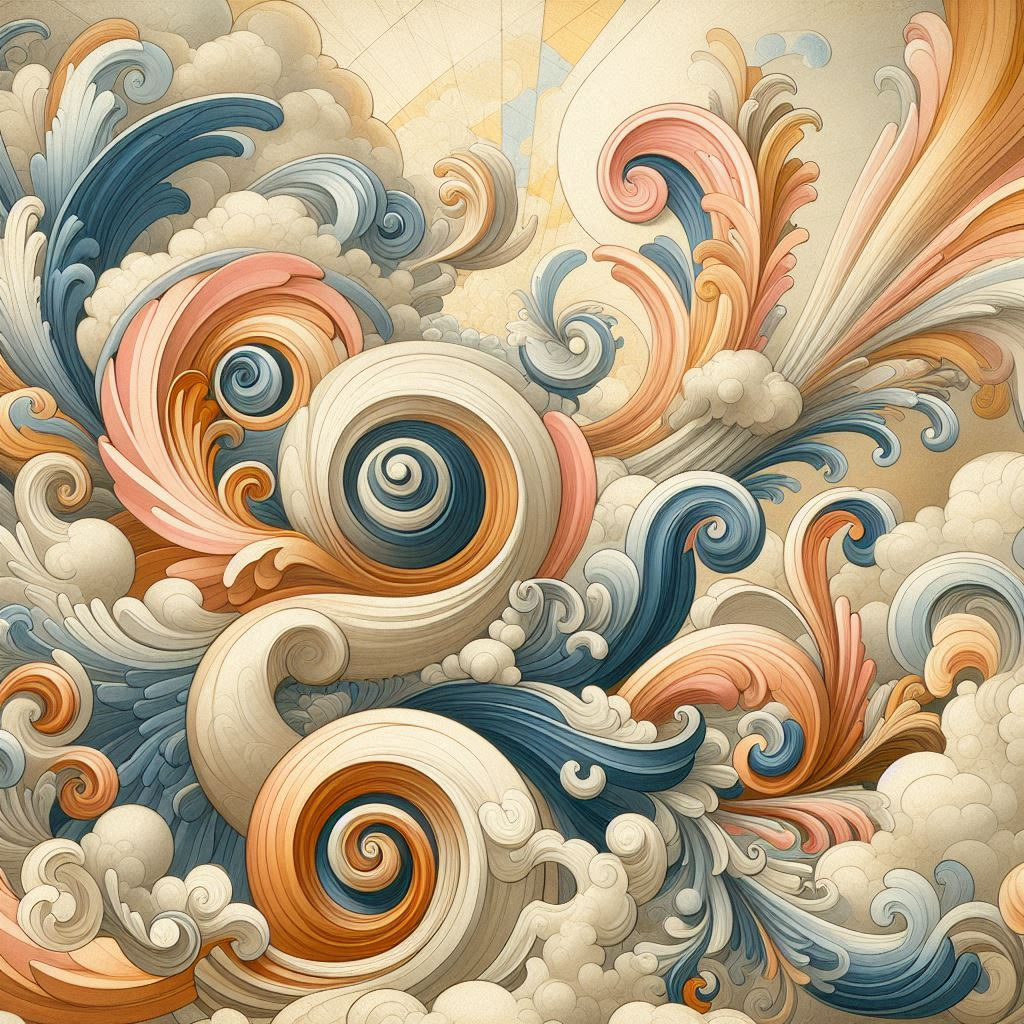
\includegraphics[trim = 18cm 5cm 8cm 10cm, clip, scale = 0.6]{pictures/page_garde.jpeg}}}
    % }
%     \ClearShipoutPicture%
%     }

%%%%%%%%%%%%%%%%%%%%%%%%%%%%%%%%%%%%%%%%%%%%%%%%%%%%%%%%%%%%%%%%%%%%%%%%
\newpage\null\thispagestyle{empty}\newpage
\cleardoublepage
\AddToShipoutPictureBG*{%
\put(2cm,18cm){
    \fbox{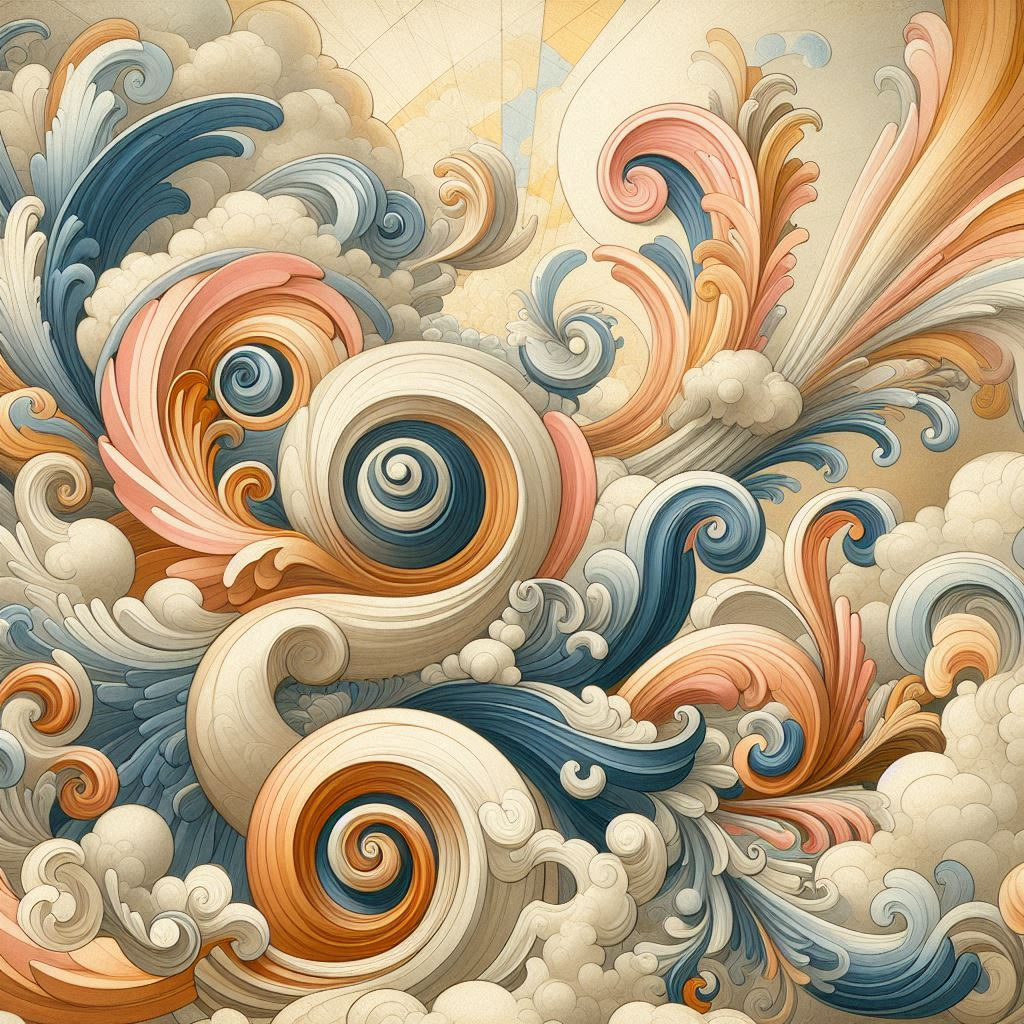
\includegraphics[trim = 0cm 0cm 27cm 27cm, clip, scale = 0.9]{pictures/page_garde.jpeg}}}
    }
    \ClearShipoutPicture%
\part{Érysichton : détecteur de failles par canal auxiliaire}

\chapter{Besoins et contraintes, préavis de conception}
\label{chap:erysichtonConception}


Ce chapitre permet de présenter le raisonnement qui a motivé la conception d'un outil de détection automatique de failles par canal auxiliaire de type temporel.

\section{Identification des besoins et spécificités}

Nous avons pu voir grâce aux chapitres précédents que la conception et l'implémentation d'un système sécurisé est un problème difficile. Une première étape est de concevoir des primitives et des protocoles mathématiquement sécurisés. Une seconde étape est de s’assurer que leurs implémentations sont effectivement sécurisées, d'un point de vue : 

\begin{itemize}
    \item mathématique contre des attaques logiques (aspect fonctionnel : le code implémente correctement les bons concepts cryptographiques)
    \item matériel, contre des attaques très bas niveau (les attaques temporelles)
\end{itemize}

Avec l'objectif de concevoir un système sûr, il nous faut donc identifier toutes les tâches à réaliser pour arriver à bout de ce projet. En plus de ce travail de planification, l'identification et l'intégration d'outils déjà implémentés nous permettra d'avancer plus rapidement vers cet objectif.\smallbreak


\subsection*{Point de départ}

En reprenant ces deux étapes, nous identifions les possibilités pour un développeur pour concevoir un système résistant à ces attaques temporelles.\smallbreak

La première étape de conception de primitives cryptologiques et de protocole n'est pas du ressort du développeur. Elle appartient aux cryptologues et aux chercheurs en sécurité mathématique. Ce sont eux qui conçoivent et maintiennent des bibliothèques cryptographiques, des boîtes à outils qui proposent les briques de sécurité nécessaires aux systèmes sécurisés.\medbreak

Plusieurs bibliothèques existent \cite{OpenSSL, BearSSL, polubelova2020haclxn} et remplissent différents objectifs :  rétrocompatiblité, politique temps constant, \etc. Notre choix est à réaliser en fonction des spécificités du produits que nous cherchons à déployer.\medbreak

La seconde étape est à distinguer en deux parties. Cette opération de vérification de la sécurité de l'implémentation peut être réalisée sur le produit fini et sur les bibliothèques employés par le produit. Comme introduit, cette étape a pour objectif la vérification formelle du code du programme et la vérification matérielle au niveau assembleur.\medbreak

Utiliser la bibliothèque \textbf{HACL*} \cite{polubelova2020haclxn, HACL*} permet d'avancer la première étape et la première partie de la seconde étape. Cette bibliothèque a été conçue formellement et vient avec les preuves mathématiques de la sécurité de son implémentation. Comme présenté en \nameref{chap:prelude}, elle est programmée en F*. Le projet permet une exploitation en C et en assembleur \cite{HACL*}.\medbreak

En revanche, la seconde étape de la seconde partie nous demande une vérification au niveau de l'assembleur. Si certaine partie de cette bibliothèque sont codées en assembleur, la majorité du projet reste du F* traduit vers C. Il faut réaliser une analyse. Dans le cadre de cette étude, l'outil d'analyse binaire retenu pour réaliser cette tâche est \textbf{Binsec}. Cet outil est implémenté en Ocaml et il est maintenu par une équipe de chercheurs et d'ingénieurs du CEA-List de Saclay.\medbreak

L'objectif est donc d'analyser HACL* dans son entièreté. Avec cette analyse complète, si elle est correcte, alors les deux étapes de réalisation d'un système sûr seront réalisées. Cela signifie qu'elle sera la première bibliothèque cryptographique formellement sûre et vérifiée résistante aux attaques temporelles.

\subsection*{Objectifs à réaliser}

Sans reprendre les explications du fonctionnement de Binsec, voir \textcolor{red}{"ref vers fonctionement de Binsec"}, l'analyse se réalise sur un fichier binaire à l'aide d'instructions à adjoindre. Avec ce point de départ, nous commençons à construire notre carnet de spécifications.

\textbf{Fichier binaire.} Il faut donc des fichiers binaires à fournir à Binsec. Or comme chacun le sait, plus un binaire est imposant, plus son analyse est difficile. Et comme Binsec emploie l'analyse symbolique, explorer un binaire imposant a un coût de mémoire quadratique sur le parcours des instructions du binaire. L'idéal est donc d'analyser plein de petits fichiers binaires.\smallbreak

\textbf{Analyse complète.} Chaque fonction de HACL* doit être analysée. En poursuivant la condition précédente, nous pouvons essayer de concevoir un binaire par fonction analysée. Nous distribuons ainsi l'analyse et nous parcourons ainsi toute les fonctions présentes dans la bibliothèque.\medbreak

\textbf{Analyse correcte.} En se rappelant comment fonctionnent les optimisations (voir le tableau \ref{tab:compile_option}) il nous faut être attentif avec certaines qui simplifient/modifient le code. Pour éviter des suppressions d'instructions, le fichier nécessite une légère contextualisation avant l'appel de la fonction analysée.

\begin{listing}[!ht]
    \caption{Code d'analyse de la fonction Hacl\_AEAD\_Chacha20Poly1305\_Simd128\-\_encrypt, testé lors de la prise en main de Binsec et HACL*}
    \label{lst:prise_en_main}
    \begin{minted}[frame=lines,framesep=2mm,baselinestretch=1.2,fontsize=\footnotesize,linenos, gobble=8]{C}
        #include <stdlib.h>

        #include "Hacl_AEAD_Chacha20Poly1305_Simd128.h"

        #define BUF_SIZE 16384
        #define KEY_SIZE 32
        #define NONCE_SIZE 12
        #define AAD_SIZE 12
        #define TAG_SIZE 16

        uint8_t plain[BUF_SIZE];
        uint8_t cipher[BUF_SIZE];
        uint8_t aead_key[KEY_SIZE];
        uint8_t aead_nonce[NONCE_SIZE];
        uint8_t aead_aad[AAD_SIZE];
        uint8_t tag[16];

        int main (int argc, char *argv[])
        {
        Hacl_AEAD_Chacha20Poly1305_Simd128_encrypt
            (cipher, tag, plain, BUF_SIZE, aead_aad, AAD_SIZE, aead_key, aead_nonce);
        exit(0);
        }
    \end{minted}
\end{listing}

De même, comme nos fichiers analysés appartiennent à la bibliothèque extérieur HACL*, l'emploi de l'option \texttt{-static} est nécessaire pour prévenir la mise place de liens vers la bibliothèque partagée dans le fichier binaire. Cette option ne nuit pas à la qualité de l'analyse, elle permet en revanche d'avoir tous les éléments sous la main lorsque nous désassemblons un fichier binaire. Retirer cette option lors de la compilation, c'est s'ajouter des lourdeurs et rallonger le temps requis pour la vérification manuelle d'un fichier.\medbreak

\textbf{Couverture de compilateur.} Les travaux de \citeauthor{schneider2024breakingbadcompilersbreak} \cite{schneider2024breakingbadcompilersbreak} ont clairement mis en évidence que le choix du compilateur est à considérer. Nous allons pouvoir identifier quel compilateur nous permet d'avoir le plus de fichiers binaires sécurisés. Cette analyse nous permet d'identifier les limites de la pratique de la programmation en temps constant.

\textbf{Couverture d'architectures.} x86\_64 et ARM sont les architectures matérielles les plus répandues dans le monde. Étendre l'analyse vers différentes plateformes et observer les différences qui émergent nous permettra d'avancer dans la direction de la conception d'une bibliothèque cryptographique universelle. Nous pouvons aussi étendre cette analyse vers d'autres architectures comme PowerPC ou RiscV.\medbreak


\textbf{Automatisation.} Faire cette analyse sur un fichier binaire, comme le code \ref{lst:prise_en_main}, avec trois axes de complexité (complétude, de la couverture d'architectures et des compilateurs) n'est pas envisageable à la main. Il faut absolument que cette analyse soit automatisée.


\section{Initialisation et tests variés}

Dans le cadre de la programmation sécuritaire, où sont développés les systèmes avec pour objectif d'un accident par siècle (métros automatiques, trains, avions\dots), les projets sont conçus selon le principe du cycle en V. Cette méthode au contraire de la méthode Agile permet de prévoir tous les cas de figure et d'usages, nous permettant de nous épargner les problèmes de correction de bogues.

\begin{figure}[!ht]
    \caption{Cycle en V}
    \label{fig:cycle_en_V}
    \centering
   \begin{tikzpicture}[
        auto,
        mynode/.style={draw, text width=2.5cm, align=center, font=\small},
        myarrow/.style={-Stealth, thick}
    ]

    % Nodes for the V-model
    \node[mynode] (req) {Besoin et exigences};
    \node[mynode, xshift=1cm, yshift=-0.5cm, below of=req] (spec) {Spécification système};
    \node[mynode, xshift=1cm, yshift=-0.5cm, below of=spec] (design) {Conception globale};
    \node[mynode, xshift=1cm, yshift=-0.5cm, below of=design] (detaildesign) {Conception détaillée};
    \node[mynode, xshift=1.3cm, yshift=-0.5cm, below of=detaildesign] (coding) {Codage et implémentation};
    \node[mynode, xshift=2cm, yshift=0.5cm, above of=coding] (unit) {Tests unitaires};
    \node[mynode, xshift=1cm, yshift=0.5cm, above of=unit] (integration) {Tests d'intégration};
    \node[mynode, xshift=1cm, yshift=0.5cm, above of=integration] (system) {Tests système};
    \node[mynode, xshift=1cm, yshift=0.5cm, above of=system] (acceptance) {Tests d'acceptation};
    \node[mynode, above of=acceptance] (maintenance) {Maintenance};

    % Arrows for the V-model
    \draw[myarrow] (req) -- (spec);
    \draw[myarrow] (spec) -- (design);
    \draw[myarrow] (design) -- (detaildesign);
    \draw[myarrow] (detaildesign) -- (coding);
    \draw[myarrow] (coding) -- (unit);
    \draw[myarrow] (unit) -- (integration);
    \draw[myarrow] (integration) -- (system);
    \draw[myarrow] (system) -- (acceptance);
    \draw[myarrow] (acceptance) -- (maintenance);

    % Arrows for the verification and validation
    \draw[myarrow, dashed, opacity=0.5] (unit.west) -- (detaildesign);
    \draw[myarrow, dashed, opacity=0.5] (integration.west) -- (design);
    \draw[myarrow, dashed, opacity=0.5] (system.west) -- (spec);
    \draw[myarrow, dashed, opacity=0.5] (acceptance.west) -- (req);

    % Legend
    \node[draw, opacity=0.5] (legend1) at (10,-2) {};
    \draw[myarrow, dashed, opacity=0.5] (legend1.east) -- ++(1,0);
    \node[anchor=west] at (11,-2) {Vérifications};

    \node[draw] (legend2) at (10,-3) {};
    \draw[myarrow] (legend2.east) -- ++(1,0);
    \node[anchor=west] at (11,-3) {Étapes successives};

    \end{tikzpicture}
\end{figure}
\begin{center}
    \rule{0.75\textwidth}{1pt}
\end{center}

Appliquer cette méthode à l'entièreté de ce projet n'est pas envisageable à cause du coût temporel qui est très élevé. Nous nous concentrons sur la réalisation d'une preuve de concept avec un produit minimal mais opérationnel. Le développement sera concentré sur l'objectif d'automatisation. Le développement d'outils permettant la réalisation des objectifs des couvertures  nécessiteront un futur travail.

\subsection*{Identification des besoins et exigences}

Nous avons déjà conçu notre carnet d'exigences. En revanche nous ne connaissons pas le comportement des outils que nous souhaitons employer. La première opération est donc de s'approprier le fonctionnement de ceux-ci. Le code \ref{lst:prise_en_main} est un exemple de test réalisé dans cette phase du projet.

Binsec est un outil uniquement utilisable au travers d'un terminal. Il s'invoque avec son alias, le binaire à analyser et les options qui seront effectuées :

\begin{listing}[!ht]
    \caption{Commande Binsec basique}
    \label{lst:commande_binsec}
    \begin{minted}{shell}
$ binsec -sse -sse-script $(BINSEC_SCRIPT) -checkct $(BINARY)
    \end{minted}
\end{listing}

L'option \texttt{-sse} permet d'activer l'analyse par exécution symbolique, \texttt{-sse-script} associé à un fichier (ici \texttt{BINSEC\_SCRIPT}) permet d'instruire notre analyse, préciser des stubs\footnote{Terme anglais du lexique de la rétro-ingénierie; module logiciel simulant la présence d'un autre.} et des initialisations. Enfin \texttt{-checkct} active la vérification de la politique temps constant au sein du fichier binaire indiqué par \texttt{BINARY}. Binsec renvoie dans le terminal le résultat de son analyse : [\texttt{secure, unknown, insecure}]. Le second est invoqué lorsque l'analyse est incomplète.\medbreak

Cette phase <<Test et Identification des exigences>> permet de confronter plusieurs fonctions de HACL* et de se familiariser avec le langage d'instructions qu'admet l'option \texttt{-sse-script}. Un tutoriel complet est accessible pour comprendre le fonctionnement l'outil Binsec depuis sa page officielle\footnote{https://binsec.github.io/}.

\begin{listing}[!ht]
    \caption{Instructions permettant de trouver le mot d'un passe d'un binaire exercice}
    \label{lst:exemple_binsec}
    \begin{minted}[frame=lines,framesep=2mm,baselinestretch=1.2,linenos]{bash}
starting from core with
  argv<64> := rsi
  arg1<64> := @[argv + 8, 8]
  size<64> := nondet            # 0 < strlen(argv[1]) < 128
  assume 0 < size < 128
  all_printables<1> := true
  @[arg1, 128] := 0
  for i<64> in 0 to size - 1 do
    @[arg1 + i] := nondet as password
    all_printables := all_printables && " " <= password <= "~"
  end
  assume all_printables
end

replace <puts>, <printf> by
return
end

reach <puts> such that @[rdi, 14] = "Good password!"
then print ascii stream password

cut at <puts> if @[rdi, 17] = "Invalid password!"

halt at <printf>
\end{minted}
\end{listing}

Ce code présenté ici est un exemple d'usage de Binsec et permet de réaliser une attaque sur un binaire issu d'une plateforme d'apprentissage à la sécurité logicielle\footnote{https://crackmes.one/}. L'exercice consiste à retrouver le mot de passe caché d'un binaire. Dans le cadre de notre exercice d'analyse de la politique temps constant, le script \ref{lst:analyse_simple_binsec} est plus simple.\medbreak

Ce script a pour objectif de vérifier les résultats apportés par \cite{schneider2024breakingbadcompilersbreak} concernant une fuite présente sur la fonction <<\textit{FStar\_UInt64\_eq\_mask}>> et d'étendre cette analyse vers d'autres architectures. Dans une première démarche d'automatisation, ce code a été généré automatiquement par un script shell. Nous pouvons voir que l'analyse ne parcourt pas l'entièreté du binaire, seulement 8 sections sont chargées (sur 24). L'analyse commence à l'appel de la fonction \texttt{main} et se termine à la ligne 8 avec une adresse de fin. Cette adresse de fin est produite par le script shell pour attraper la fin de la fonction \texttt{main}. 

\begin{listing}[!ht]
    \caption{Instructions permettant d'analyser le code \ref{lst:Hacl_masking} compilé vers RiscV-32}
    \label{lst:analyse_simple_binsec}
    \begin{minted}[frame=lines,framesep=2mm,baselinestretch=1.2,linenos]{bash}
load sections .plt, .text, .rodata, .data, .got, .got.plt, .bss from file

secret global  r, cin, y, x

starting from <main>

with concrete stack pointer
halt at  0x0000000000000464
explore all

\end{minted}
\end{listing}


Ce modèle, qui nous servira de base pour la suite du développement, a permis une analyse rapide entre différents compilateurs et différentes architectures.

\subsection*{Application et observation entre architectures et compilateurs}


\begin{figure}[!ht]
    \caption{Tableau de résultats d'analyse Binsec pour architecture ARMv7 et ARMv8}
    \label{tab:resultats_arm}
    \begin{center}    
        \begin{tabular}{|c|c|c|c|c|c|}
            \hline
            \rowcolor{blue!10}
            \cellcolor{inria-2024-gris-bleu!20}\textbf{opt}\textbackslash\textbf{fonction analysée} & \multicolumn{5}{c|}{\textbf{cmovznz4}} \\
            \hline
            \rowcolor{blue!30}
            \textbf{Clang+LLVM} & \textbf{14.0.6} & \textbf{15.0.6} & \textbf{16.0.4} & \textbf{17.0.6} & \textbf{18.1.8} \\
            \hline
            \rowcolor{orange!30!red!50}
            \textbf{-O0} & \cellcolor{green!60}\checkmark & \cellcolor{green!60}\checkmark & \cellcolor{green!60}\checkmark  & \cellcolor{green!60}\checkmark  & \cellcolor{green!60}\checkmark  \\
            \hline
            \rowcolor{orange!30!red!50}
            \textbf{-O1} & \cellcolor{green!60}\checkmark & \cellcolor{green!60}\checkmark & \cellcolor{green!60}\checkmark  & \cellcolor{green!60}\checkmark  & \cellcolor{green!60}\checkmark  \\
            \hline
            \rowcolor{orange!30!red!50}
            \textbf{-O2} & \cellcolor{green!60}\checkmark & \cellcolor{green!60}\checkmark & \cellcolor{green!60}\checkmark  & \cellcolor{green!60}\checkmark  & \cellcolor{green!60}\checkmark  \\
            \hline
            \rowcolor{orange!30!red!50}
            \textbf{-O3} & \cellcolor{green!60}\checkmark & \cellcolor{green!60}\checkmark  & \cellcolor{green!60}\checkmark  & \cellcolor{green!60}\checkmark  & \cellcolor{green!60}\checkmark  \\
            \hline
            \rowcolor{orange!30!red!50}
            \textbf{-Os} & \cellcolor{green!60}\checkmark  & \cellcolor{green!60}\checkmark  & \cellcolor{green!60}\checkmark  & \cellcolor{green!60}\checkmark  & \cellcolor{green!60}\checkmark  \\
            \hline
            \rowcolor{orange!30!red!50}
            \textbf{-Oz} & \cellcolor{green!60}\checkmark  & \cellcolor{green!60}\checkmark  &  \cellcolor{green!60}\checkmark  &  \cellcolor{green!60}\checkmark  &  \cellcolor{green!60}\checkmark \\
            \hline
        \end{tabular}   
    \end{center}
    \raggedleft
    \small{
    \checkmark : \textit{binary secure}
    }
\end{figure}

Nous comprenons, à la lecture du tableau \ref{tab:resultats_arm}, que la politique temps constant est considérée respectée par Binsec sur les versions testées ainsi que pour les différentes options de compilation. Ce résultat est encourageant pour la suite du projet.\medbreak

\begin{figure}[!htb]
    \caption{Tableau de résultats d'analyse Binsec pour architecture Risc-V}
    \label{tab:resultats_riscv}
    \begin{center}

    \begin{tabular}{|c|cc|cc|}
        \hline
        \rowcolor{blue!10}
        \cellcolor{inria-2024-gris-bleu!20}\textbf{opt}\textbackslash\textbf{fonction analysée} & \multicolumn{2}{c|}{\textbf{cmovznz4} - 64 bits} & \multicolumn{2}{c|}{\textbf{cmovznz4} - 32 bits} \\
        \hline
        \rowcolor{blue!30}
        \textbf{Compilateur et architecture} & gcc 15.1.0 & clang 19.1.7 & gcc 15.1.0& clang 19.1.7 \\
        \hline
        \rowcolor{orange!30!red!50}
        \textbf{-O0} &  \cellcolor{orange!60}\textasciitilde  & \cellcolor{red!60}$\times$ & \cellcolor{orange!60}\textasciitilde & \cellcolor{red!60}$\times$ \\
        \hline
        \rowcolor{orange!30!red!50}
        \textbf{-O1} &  \cellcolor{green!60}\checkmark & \cellcolor{red!60}$\times$ & \cellcolor{green!60}\checkmark & \cellcolor{red!60}$\times$ \\
        \hline
        \rowcolor{orange!30!red!50}
        \textbf{-O2} &  \cellcolor{green!60}\checkmark & \cellcolor{red!60}$\times$ & \cellcolor{green!60}\checkmark & \cellcolor{red!60}$\times$ \\
        \hline
        \rowcolor{orange!30!red!50}
        \textbf{-O3} &  \cellcolor{green!60}\checkmark & \cellcolor{red!60}$\times$ & \cellcolor{green!60}\checkmark & \cellcolor{red!60}$\times$ \\
        \hline
        \rowcolor{orange!30!red!50}
        \textbf{-Os} &  \cellcolor{green!60}\checkmark & \cellcolor{red!60}$\times$ & \cellcolor{green!60}\checkmark & \cellcolor{red!60}$\times$ \\
        \hline
        \rowcolor{orange!30!red!50}
        \textbf{-Oz} &  \cellcolor{green!60}\checkmark & \cellcolor{red!60}$\times$ & \cellcolor{green!60}\checkmark & \cellcolor{red!60}$\times$ \\
        \hline
    \end{tabular}
    \end{center}
    \raggedleft
     \small{
        \checkmark : \textit{binary secure} ;
        \textasciitilde : \textit{binary unknown} ;
        $\times$ : \textit{binary insecure}
    }
\end{figure}

Les résultats dans le tableau \ref{tab:resultats_riscv} sont indéniables : la version 19.1.7 de clang rend le code source perméable à des attaques temporelles.\medbreak

\begin{CitationBox}{Identification de défaut}
    Pour construire le tableau \ref{tab:resultats_riscv}, plusieurs alertes se sont levées et ont permis de mettre en évidence un bug présent dans Binsec. Cette erreur dans l'analyse symbolique provoquait l'arrêt de l'exploration par explosion de l'usage de la mémoire. Les registres \texttt{ld} (\textit{load}) et \texttt{sd} (\textit{store}) étaient mal gérés. En particulier l'opérande \texttt{ld}, simulé par un tableau, n'était jamais vidé. Cette découverte a amené un correctif et une amélioration de Binsec. De par l'envergure de ce projet, il est possible que d'autres erreurs dues à Binsec soient découvertes. L'exploration de nombreuses et nouvelles ISA\footnote{Acronyme anglais pour Architecture de Jeu d'Instruction, désigne l'ensemble des instructions assembleur associées à une architecture.}, surtout avec Risc-V qui est encore en développement et perfectionnement, permet de renforcer cet outil plus efficacement et rapidement que par la conception de tests manuels.\medbreak
\end{CitationBox}
    
    


En explorant plus en avant le code binaire, nous découvrons que ces erreurs sont dues à l'opérande \texttt{beqz}\footnote{Effectue un branchement si la valeur du registre consulté est zéro. Cette opérande est propre à Risc-V.}. L'ISA de Risc-V n'a pas à sa disposition un opérande comme \texttt{cmov} en X86\_64 ou ARM. Donc l'application d'optimisation de compilation force l'usage de cette opérande qui n'est pas en temps constant. L'optimisation qui réalise ce changement se nomme <<\textit{InstCombinePass}>>.\medbreak

Nous observons ici une manifestation indéniable des précédents résultats proposés par d'autres travaux de recherche. Une solution serait de modifier l'ISA pour permettre cette opération d'être en temps constant. Celle qui a été retenue, c'est d'employer un \texttt{pragma}, ici \texttt{\# pragma clang optimise <off/on>}. Cette instruction, donnée dans le code source, indique au compilateur de désactiver ses optimisations pour le code contenu entre les deux balises \texttt{off,on}. Cette solution entraîne des pertes de performance et des ralentissements quant au temps de compilation et à l'usage des ressources. Il est donc préférable de l'utiliser avec parcimonie.\medbreak

Après avoir ciblé notre besoin, les exigences associées et effectué des tests pour comprendre le processus à automatiser, nous pouvons synthétiser la démarche avec la figure \ref{fig:compilation_simple} : depuis HACL*, nous extrayons une fonction qui sera testé, nous fabriquons le fichier de test en C; nous identifions les paramètres secrets et nous concevons le script adéquat pour Binsec; nous compilons le fichier C à notre guise et nous terminons par l'analyse Binsec.

\begin{figure}[!ht]
    \caption{Flot de travail de l'outil d'analyse à concevoir}
    \label{fig:compilation_simple}
    \centering
    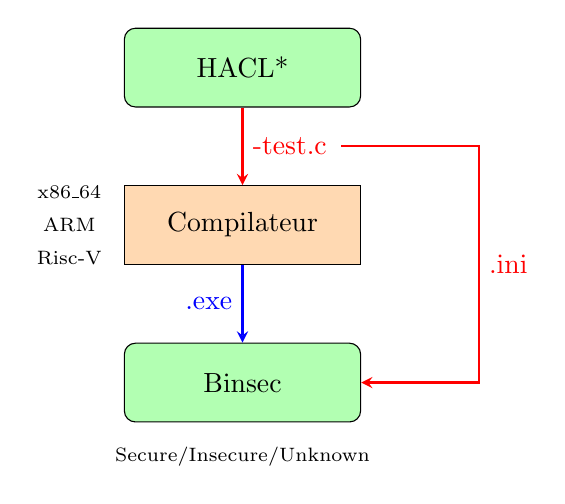
\begin{tikzpicture}[node distance=2cm]

    % Styles des noeuds
    \tikzstyle{startstop} = [rectangle, rounded corners, minimum width=3cm, minimum height=1cm,text centered, draw=black, fill=green!30]
    \tikzstyle{process} = [rectangle, minimum width=3cm, minimum height=1cm, text centered, draw=black, fill=orange!30]
    \tikzstyle{intermediate} = [circle, minimum size=0.5cm, text centered, draw=white, fill=white]
    \tikzstyle{arrow} = [thick,->,>=stealth]
    
    % Noeuds
    \node (hacl) [startstop] {HACL*};
    \node (inter) [intermediate, below of=hacl,xshift=1cm, yshift=1cm] {};
    \node (compilateur) [process, below of=hacl] {Compilateur};
    \node (binsec) [startstop, below of=compilateur] {Binsec};
    
    % Flèches
    \draw [arrow, red] (hacl) -- node[anchor=west] {-test.c} (compilateur);
    \draw [arrow, red] (inter) -- ++(2,0) |- node[anchor=west, pos=0.25] {.ini} (binsec);
    \draw [arrow, blue] (compilateur) -- node[anchor=east] {.exe} (binsec);
    
    % Annotations
    \node[align=center, left of=compilateur, xshift=-0.2cm] {\scriptsize x86\_64\\ \scriptsize ARM\\ \scriptsize Risc-V};
    \node[align=center, below of=binsec, yshift=30pt] {\scriptsize Secure/Insecure/Unknown};
    
    \end{tikzpicture}

\end{figure}

\vfill
\textit{Nous allons maintenant nous pencher sur le procédé de conception de notre outil de détection automatique de failles temporelles.}






\chapter{Érysichthon à jamais affamé}
\label{chap:erysichtonUsage}

intro


\section{Planification et préparations}

Nous avons nos spécificités techniques et nous savons qu'elle forme notre outil doit avoir (fig \ref{fig:compilation_structure}). Nous pouvons commencer par synthétiser les opérations nécessaires.\smallbreak

Nous allons donc concevoir des protocoles pour identifier les étapes nécessaires pour que Binsec analyse entièrement un fichier et nous renvoie un parmi [\texttt{secure, unknown, insecure}]. Le protocole \texttt{x86\_64} est particulier. Depuis la version \textbf{0.5.0} de Binsec il est possible de fournir un <<cliché mémoire>>\footnote{Plus couramment 'Core dump', terme technique anglais désignant une copie de la mémoire vive et des registres d'un programme. Ce fichier sert à être analysé, généralement par un débogueur.} pour accélérer l'analyse. Nous utilisons cet avantage pour l'intégrer à notre graphe d'éxécution. La machine sur laquelle le projet sera développé est sur une architecture x86\_64, cela nous permet d'utiliser l'outil GDB pour la génération de cliché mémoire.\medbreak

\begin{figure}[!ht]
    \caption{Protocole pour analyser des fichiers compilés en x86\_64}
    \label{fig:protocole_x86}
    \centering
  \begin{tikzpicture}[auto]

    % Styles
    \tikzstyle{startstop} = [rectangle, rounded corners, minimum width=2cm, minimum height=1cm, text centered, draw=black, fill=green!30]
    \tikzstyle{process} = [rectangle, minimum width=2cm, minimum height=1cm, text centered, draw=black, fill=orange!30]
    \tikzstyle{arrow} = [thick,->,>=stealth]
    \tikzset{zone1/.style={rectangle, rounded corners, draw=red, dashed, fill=red!10, inner sep=0.3cm}}
    \tikzset{zone2/.style={rectangle, rounded corners, draw=blue, dashed, fill=blue!10, inner sep=0.3cm, opacity = 0.7}}
    \tikzset{zone22/.style={rectangle, rounded corners, draw=none, fill=blue!10, inner sep=0.3cm}}
    \tikzset{zone3/.style={rectangle, rounded corners, draw=green, dashed, fill=green!10, inner sep=0.3cm}}
    
    % Noeuds
    \node (hacl) [startstop] {Hacl*};
    \node (c) [below of=hacl] {Fonction};
    \node (ini) [below of=c, xshift=2cm] {.ini};
    \node (test) [below of=c, xshift=-2cm] {-test.c};
    \node (script) [below of=c] {.script};
    \node (compilateur) [process, below of=test] {Compilateur};
    \node (exe) [below of=compilateur] {-test.exe};
    \node (blanc1) [below of=script] {};
    \node (blanc2) [below of=blanc1] {};
    \node (gdb) [process, below of=blanc2] {GDB};
    \node (snap) [right of=gdb, xshift=2cm] {.snapshot};
    \node (binsec) [startstop, right of=snap, xshift=1.5cm] {Binsec};
    
    % Flèches
    \draw [arrow] (hacl) -- (c);
    \draw [arrow] (c) -- (ini);
    \draw [arrow] (c) -- (test);
    \draw [arrow] (c) -- (script);
    \draw [arrow] (test) -- (compilateur);
    \draw [arrow] (compilateur) -- (exe);
    \draw [arrow] (exe) -- (gdb);
    \draw [arrow] (script) -- (gdb);
    \draw [arrow] (gdb) -- (snap);
    \draw [arrow] (snap) -- (binsec);
    \draw [arrow] (ini) -- (binsec);

    % Zones
    \begin{scope}[on background layer]
        \node [zone1, fit=(c) (ini) (test) (script)] {};
        \node [zone2, fit=(script) (gdb)] {};
              \node [zone2, fit=(gdb) (snap) (binsec)] {};
              \draw [zone22]
              ([xshift=-10pt, yshift=10pt]gdb.north west) --
              ([xshift=10pt, yshift=10pt]gdb.north east) -- 
              ([xshift=10pt, yshift=-9pt]gdb.south east) -- 
              ([xshift=1pt, yshift=-1pt]gdb.south west) --
              cycle;  
    \node [zone3, fit=(compilateur) (exe)] {};
    \end{scope}
    \end{tikzpicture}
\end{figure}

Ce graphe modélise la chaîne d'étapes nécessaire à l'obtention d'une analyse Binsec pour une fonction que nous ciblons. Plusieurs zones sont distinguées. La zone verte correspond à l'étape de compilation, la zone bleue à l'étape de préparation de l'analyse et la zone rouge à la synthèse de fichiers (de tests et d'instruction pour l'analyse de Binsec). Ce choix de couleur est adapté à la difficulté attendue de chaque étape. L'opération de compilation consiste en une commande. L'opération de préparation d'analyse consiste simplement en deux commandes : un appel à GDB avec le binaire puis un appel à Binsec avec le cliché mémoire et les instructions d'analyse.\smallbreak

Avec ce graphe réalisé, nous pouvons le modifier pour préparer la voie à d'autres architectures. Dans un format plus générique voici comment se présente le protocole d'analyse :

\begin{figure}[!ht]
    \caption{Protocole générique d'analyse}
    \label{fig:protocole_generique}
    \centering
  \begin{tikzpicture}[auto]

    % Styles
    \tikzstyle{startstop} = [rectangle, rounded corners, minimum width=2cm, minimum height=1cm, text centered, draw=black, fill=green!30]
    \tikzstyle{process} = [rectangle, minimum width=2cm, minimum height=1cm, text centered, draw=black, fill=orange!30]
    \tikzstyle{arrow} = [thick,->,>=stealth]
    \tikzset{zone1/.style={rectangle, rounded corners, draw=red, dashed, fill=red!10, inner sep=0.3cm}}
    \tikzset{zone2/.style={rectangle, rounded corners, draw=blue, dashed, fill=blue!10, inner sep=0.3cm, opacity = 0.5}}
    \tikzset{zone3/.style={rectangle, rounded corners, draw=green, dashed, fill=green!10, inner sep=0.3cm}}
    
    % Noeuds
    \node (hacl) [startstop] {Hacl*};
    \node (c) [below of=hacl] {Fonction};
    \node (ini) [below of=c] {.ini};
    \node (test) [below of=c, xshift=-2cm] {-test.c};
    \node (compilateur) [process, below of=test] {Compilateur};
    \node (exe) [below of=compilateur] {-test.exe};
    \node (blanc) [below of=c] {};
    \node (blanc1) [below of=blanc] {};
    \node (blanc2) [below of=blanc1] {};
    \node (binsec) [startstop, below of=blanc2] {Binsec};
    
    % Flèches
    \draw [arrow] (hacl) -- (c);
    \draw [arrow] (c) -- (ini);
    \draw [arrow] (c) -- (test);
    \draw [arrow] (test) -- (compilateur);
    \draw [arrow] (compilateur) -- (exe);
    \draw [arrow] (exe) -- (binsec);
    \draw [arrow] (ini) -- (binsec);

    % Zones
    \begin{scope}[on background layer]
        \node [zone1, fit=(c) (ini) (test) ] {};
        \node [zone2, fit=(ini) (binsec)] {};
        \node [zone3, fit=(compilateur) (exe)] {};
    \end{scope}    
    \end{tikzpicture}
\end{figure}

Dans ce contexte, une question se pose : est-ce que la conception des scripts pour Binsec (\textit{.ini}) est automatisable ou est-ce qu'il faudra utiliser des émulateurs pour générer des clichés mémoire et revenir dans le cas de la figure \ref{fig:protocole_x86} ?\smallbreak

En effet, l'importance de cette question se révèle lorsque nous changeons d'architecture et que nous devons nous passer de clichés mémoire. Sur notre machine en x86\_64, si nous analysons un fichier compilé en ARM, alors nous pouvons rencontrer des appels à des fonctions systèmes : les \texttt{IFUNC}. Or la résolution de ces fonctions est gérée dynamiquement lors de l'exécution du programme. Cette mécanique permet d'utiliser des implémentations optimisées en fonction des configurations du système d'éxécution. Or comme Binsec réalise une analyse symbolique du programme, il faut lui spécifier quelles fonctions correspondent aux \texttt{IFUNC} qu'il peut croiser. pour illustrer ce point, observons le script nécessaire pour une vérification de la fonction <<Hacl \_AEAD \_Chacha20Poly1305\_Simd128\_encrypt>> compilé vers ARMv8.

\begin{listing}[!ht]
    \caption{Script d'instruction pour analyser un binaire compilé vers ARM}
    \label{lst:script_arm_exemple}
    \begin{minted}{bash}
load sections .plt, .text, .rodata, .data, .got, .got.plt, .bss from file

secret global input1, aad1

@[0x00000048f008 ,8] := <__memcpy_generic>
@[0x00000048f018, 8] := <__memset_generic>
@[0x00000048f030 ,8] := <__memcpy_thunderx2>

starting from <main>
with concrete stack pointer


halt at <exit>
explore all 
    \end{minted}
\end{listing}

Les lignes 5 à 7 sont présentes pour indiquer les branchements à effectuer par Binsec lorsqu'il rencontre ces adresses. Cette opération automatiquement exécutée lors de l'initialisation de l'exécution doit ici être précisée avec les fonctions présentes dans le binaire. Automatiser ces affectations peut être difficile et nécessiter quelques outils d'analyse supplémentaires pour attraper les adresses qui ont besoin d'être réaffectées et leur attribuer les fonctions les plus adaptées.\medbreak


\begin{CitationBox}{Nommer un outil}
    Rapidement il a fallu trouver un nom pour ce projet, l'appeler par "Notre outil\dots" devenait lourd et redondant entre les réunion hebdomadaire. En revanche trouver LE nom adéquat n'est pas une chose aisée, il peut être dû à une blague, une référence ou plus simplement lié au sens du projet. Dans notre cas, nous aimons la mythologie et le travail réalisé peut se résumer à "faut donner à manger à Binsec".\smallbreak
    Érysichthon est un personnage de la mythologie grecque condamné à être affamé au point de se dévorer lui-même pour avoir détruit l'idole d'un dieu. Ce nom me plaît et sera retenu pour la suite du projet. 
\end{CitationBox}

\subsection*{Conception d'Érysichthon}


Nous avons vu les protocoles nécessaires pour construire une analyse complète. Nous avons fait des tests pour comprendre le fonctionnement de Binsec et comment doivent être déclarées les fonctions de Hacl*. Nous passons donc en phase de conception et construisons notre outil \textit{Érysichthon}. Il sera une combinaison de script Python, script shell et de Makefile. Nous appelons module un ensemble de script qui réalise une tâche au sein d'\textit{Érysichthon}. Nous vous présentons en figure \ref{fig:erysichthon} comment s'organisent les modules et les tâches qu'ils effectuent.

\begin{figure}[!ht]
    \caption{Structure des modules d'Érysichthon}
    \label{fig:erysichton}
    \centering
    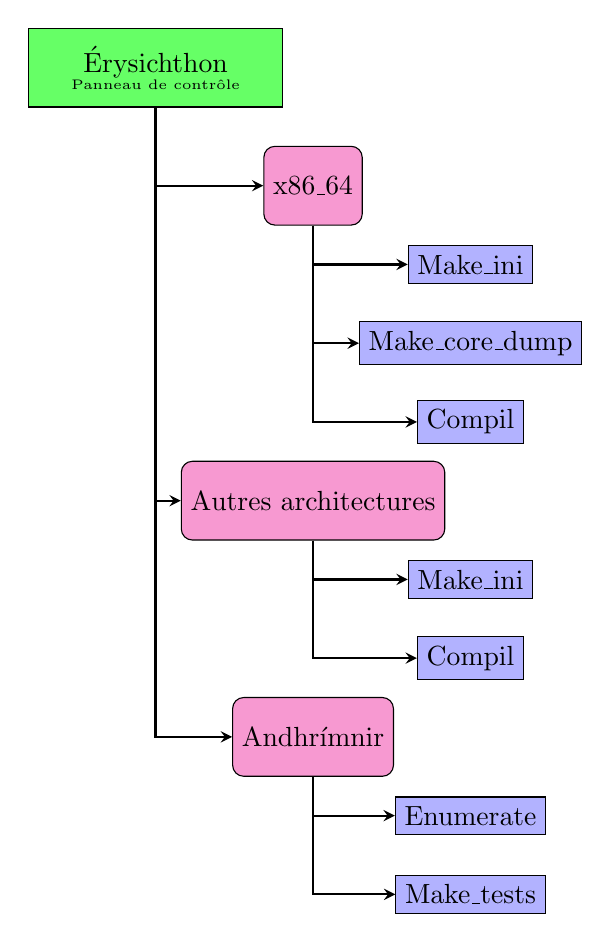
\begin{tikzpicture}[auto]

    % Styles
    \tikzstyle{startstop} = [rectangle, minimum width=2cm, minimum height=1cm, text centered, draw=black, fill=green!60]
    \tikzstyle{process} = [rectangle, rounded corners,minimum width=1cm, minimum height=1cm, text centered, draw=black, fill=magenta!40]
     \tikzstyle{process2} = [rectangle, minimum width=0.8cm, minimum height=0.3cm, text centered, draw=black, fill=blue!30]
    \tikzstyle{arrow} = [thick,->,>=stealth]
    
    % Noeuds
    \node (control) [startstop] {\parbox{3cm}{\centering Érysichthon \\ \tiny{Panneau de contrôle}}};
    \node (x86) [process, below of=control, xshift= 2cm, yshift=-0.5cm] {x86\_64};
    \node (x86-ini) [process2, below of=x86, xshift = 2cm] {Make\_ini};
    \node (x86-dump) [process2, below of=x86-ini] {Make\_core\_dump};
    \node (x86-compil) [process2, below of=x86-dump] {Compil};
    \node (arm) [process, below of=x86-compil, xshift=-2cm] {Autres architectures};
    \node (arm-ini) [process2, below of=arm, xshift=2cm] {Make\_ini};
    \node (arm-compil) [process2, below of=arm-ini] {Compil};
    \node (test) [process, below of=arm-compil, xshift=-2cm] {Andhrímnir};
    \node (enum) [process2, below of=test, xshift=2cm] {Enumerate};
    \node (exe) [process2, below of=enum] {Make\_tests};

    % Flèches
    \draw [arrow] (control) -- ++(0,-1.5) -- (x86);
    \draw [arrow] (control) -- ++(0,-5.5) -- (arm);
    \draw [arrow] (control) -- ++(0,-8.5) -- (test);
    \draw [arrow] (x86) -- ++(0,-1) -- (x86-ini);
    \draw [arrow] (x86) -- ++(0,-2) -- (x86-dump);
    \draw [arrow] (x86) -- ++(0,-3) -- (x86-compil);
    \draw [arrow] (arm) -- ++(0,-1) -- (arm-ini);
    \draw [arrow] (arm) -- ++(0,-2) -- (arm-compil);
    \draw [arrow] (test) -- ++(0,-1) -- (enum);
    \draw [arrow] (test) -- ++(0,-2) -- (exe);
    
    \end{tikzpicture}
\end{figure}

Nous retrouvons les différentes étapes de nos protocoles représentées par des rectangles symbolisant les modules associés depuis leurs noeuds respectifs : <<\texttt{Make\_ini}>> pour la génération des scripts pour Binsec, <<\texttt{Make\_core\_dump}>> pour la génération des clichés mémoires et <<\texttt{Compil}>> pour les appels aux compilateurs. Le dernier noeud <<\texttt{Andhrímnir}>> est particulier et détaillé dans la section suivante. 

\subsection*{Andhrímnir}

Ce module de Érysichthon est particulier car il est lui aussi baptisé. Ce module consiste à produire les fichiers qui seront compilés puis analysés par Binsec. Son nom est celui du cuisinier des dieux de la mythologie nordique, un travail répétitif et quotidien qu'il réalise ici pour notre outil.\smallbreak

Ce module est nommé car il constitue un projet dans le projet, sa conception seule a pris plus de la moitié du temps de développement total. C'est un outil qui, à partir d'un projet en C, est capable de générer automatiquement des tests qui compilent et peuvent ensuite être proposé à des outils d'analyse binaire. Ce module est aggrégé à Érysichthon mais peut être porté vers d'autre projets. À la différence des logiciels qui produisent des tests unitaires ( uniquement sur des projet Java, Haskell ou C\# et souvent associé à des offres payantes), il y a ici une garantie quant à la complétude des tests produit. Toutes les fonctions présentes dans le projet C analysé auront un test associé.\smallbreak

Ce module, comme son grand frère, est fonctionnel et abouti. En revanche, il nécessite quelques opérations manuelles supplémentaires et quelques améliorations pour pouvoir supporter n'importe quel projet C. Additionnellement il possède quelques optimisations propres à Hacl* permettant d'accélérer la mise en service d'Érysichthon.

\section{Conception et usages}

Nous commençons par le petit frère, Andhrímnir. Il fonctionne avec une phase d'initialisation <<\texttt{Enumerate}>> et une phase de production de tests <<\texttt{Make\_tests}>>, elle-même découpée en plusieurs étapes. La génération de \textbf{548} fichiers de tests est réalisé en moins de deux secondes.\smallbreak

\subsection*{Enumerate}

Cette étape, de réalisation très simple, consiste à identifier toutes les fonctions qui auront un fichier test généré. Comme Hacl* génère automatiquement son code C, nous exploitons cette particularité pour lister efficacement nos fonctions. L'opération actuellement réalisée est de lister l'ensemble des fichiers "\textbf{.h}" contenu dans le répertoire cible. Ensuite un parcours et une lecture de ceux-ci nous donne toutes les fonctions de l'API d'Hacl* et d'avoir une couverture complète du projet.\smallbreak

C'est lors de cette étape que nous spécifions les fonctions à tester (ou nous pouvons aussi retirer des fonctions de la chaîne de production). Ce garde-fou permet d'accélérer l'obtention des résultats finaux et d'aider grandement lorsque nous souhaitons déboguer.

\subsection*{Make\_test}

Le modèle de fichier que nous construisons est similaire aux tests minimaux préalablement réalisés. Des paramètres, une déclaration de fonction et un appel à la fonction \texttt{exit}, c'est notre recette pour une analyse simple. Binsec réalise une analyse symbolique, il ignore donc la valeur réelle des entrées. Notre objectif avec notre recette est de concevoir un test qui compile et qui contient toutes les instructions assembleurs qui pourront être analysées. L'exemple \ref{fig:gen_test_simple} illustre comment sont générés nos fichiers de tests.\medbreak

\begin{figure}[!ht]
  \caption{Test de la fonction Hacl\_EC\_K256\_felem\_sqr}
  \label{fig:gen_test_simple}
  \begin{minted}{c}
//
// Made by
// ANDHRÍMNIR - 0.3.0
// 09-07-2025
//

#include <stdlib.h>
#include "Hacl_EC_K256.h"

#define BUFFER_SIZE 5
uint64_t a[BUFFER_SIZE];
uint64_t out[BUFFER_SIZE];


int main (int argc, char *argv[]){
Hacl_EC_K256_felem_sqr(a, out);
  exit(0);
}   
  \end{minted}

  \begin{tikzpicture}[overlay , remember picture, node distance=0.5cm]
    
    \tikzset{intro/.style={rectangle, rounded corners, draw=green, fill=green!50, inner sep=0.3cm, opacity=0.2, font=\bfseries}}
    \tikzset{definition/.style={rectangle, rounded corners, draw=blue, fill=blue!50, inner sep=0.3cm, opacity=0.2, font=\bfseries}}
    \tikzset{main/.style={rectangle, rounded corners, draw=orange, fill=orange!50, inner sep=0.3cm, opacity=0.2, font=\bfseries}}
    \tikzset{labelshift/.style={xshift=3cm, yshift=0.5cm}}

    \node[intro, fit={(0,8) (12.2,5.1)}, label={[labelshift]center:Phase introductive : 8 lignes}]{};
    \node[definition, fit={(0,3) (12.2,4.5)}, label={[labelshift]center:Phase déclarative}]{};
    \node[main, fit={(0,1) (12.2,2.3)}, label={[labelshift]center:Phase principale}]{};

  \end{tikzpicture}
\end{figure}

Une première partie initie le fichier. Cette partie contient les appels inclusifs de la bibliothèque standard C, l'invocation de la bibliothèque Hacl* au travers du fichier d'en-tête de référence (ici \texttt{Hacl\_EC\_K256}) et la signature de fabrication en commentaire. L'utilisation de la bibliothèque standard permet d'utiliser la fonction \texttt{exit}. Avec cet appel, nous construisons nos scripts Binsec avec une interruption sur cette fonction. Cet arrêt précoce permet d'accélérer l'analyse du binaire de la cible (ici \texttt{Hacl\_EC\_K256\_felem\_sqr}) et nous garantit que cette analyse soit complète.\smallbreak

La deuxième partie contient tous les éléments déclaratifs nécessaires à l'invocation de la fonction. Puis se termine avec le corps du fichier C qui contient l'appel de la fonction, notre balise de fin avec la fonction \texttt{exit}. Cette construction est standardisée entre les fichiers et permet de mettre en place quelques optimisations.


\begin{figure}[!ht]
    \caption{Schéma de conception d'Andhrímnir}
    \label{fig:schema_andrhimnir}
    \centering
    \begin{adjustwidth}{-10mm}{0mm}
    \begin{tikzpicture}[auto]
    % Définition des styles pour les boîtes et flèches
    \tikzset{
      box1/.style={rectangle, draw=black, fill=cyan!30, thick, rounded corners, minimum width=2.5cm, minimum height=1cm, align=center},
      box2/.style={rectangle, draw=black, fill=orange!30, thick, rounded corners, minimum width=2.5cm, minimum height=1cm, align=center},
      box3/.style={rectangle, draw=black, fill=yellow!30, thick, rounded corners, minimum width=2.5cm, minimum height=1cm, align=center},
      box4/.style={rectangle, draw=black, fill=green!30, thick, rounded corners, minimum width=2.5cm, minimum height=1cm, align=center},
      box5/.style={rectangle, draw=black, fill=blue!30, thick, rounded corners, minimum width=2.5cm, minimum height=1cm, align=center},
      box6/.style={rectangle, draw=black, fill=magenta!30, thick, rounded corners, minimum width=2.5cm, minimum height=1cm, align=center},
      box65/.style={rectangle, draw=black, fill=magenta!60, thick, rounded corners, minimum width=1.5cm, minimum height=0.6cm, align=center},
      box7/.style={rectangle, draw=black, fill=red!30, thick, rounded corners, minimum width=2.5cm, minimum height=1cm, align=center},
      box8/.style={rectangle, draw=black, fill=blue!45, thick, rounded corners, minimum width=2.5cm, minimum height=1cm, align=center},
      arrow1/.style={->, thick, color=cyan!70!black},
      arrow2/.style={->, thick, color=orange!80!black},
      arrow3/.style={->, thick, color=yellow!80!black},
      arrow4/.style={->, thick, color=green!80!black},
      arrow5/.style={->, thick, color=blue!80!black},
      arrow6/.style={->, thick, color=magenta!80!black},
      arrow7/.style={->, thick, color=red!80!black},
      arrow8/.style={->, thick, color=gray!80!black}
      }
      \tikzset{zone1/.style={rectangle, rounded corners, draw=blue, dashed, fill=blue!10, inner sep=0.5cm, text width=3cm}}

    % Noeuds principaux (ligne du haut)
    \node[] (build_test) at (0,0) {};
    \node[box2, below of=build_test] (parse_h) {Lecture du .h};
    \node[box3, right=1cm of parse_h] (read_json) {Lecture .json};
    \node[box4, right=1cm of read_json] (build_local_json) {Accumulation d'informations};

    % Ligne du bas (génération du .c)
    \node[box5, below=1cm of build_local_json] (build_intro) {Gen. introduction};
    \node[box6, left=1cm of build_intro] (build_def) {Gen. déclaration};
    \node[box7, left=1cm of build_def] (add_main) {Gen. main};
    \node[box8, left=1cm of add_main] (fichier_c) {fichier .c};

    % Flèches horizontales principales
    \draw[arrow1] (build_test) -- (parse_h);
    \draw[arrow2] (parse_h) -- (read_json);
    \draw[arrow3] (read_json) -- (build_local_json);
    \draw[arrow4] (build_local_json) -- (build_intro);
    \draw[arrow5] (build_intro) -- (build_def);
    \draw[arrow6] (build_def) -- (add_main);
    \draw[arrow7] (add_main) -- (fichier_c);

    % Branche auxiliaire depuis build introduction
    \node[box5, left of = build_intro, yshift=-1cm] (detect_aux) {Détection appel auxiliaire};
    % Ajout de deux barres obliques sur la flèche build_intro -> build_def
    \draw[thick] ($(build_intro)!0.5!(build_def) + (0,0.3)$) -- ($(build_intro)!0.5!(build_def) + (0,-0.54)$);
    \draw[thick] ($(build_intro)!0.55!(build_def) + (0,0.3)$) -- ($(build_intro)!0.55!(build_def) + (0,-0.54)$);


    \node[box3, left=1cm of detect_aux, yshift=-2cm] (test_exist) {test si fichier existe};
    \draw[arrow5] (detect_aux) -- (test_exist);

    % Oui -> Collage -> build definition
    \node[box4, above of = test_exist, yshift=0.5cm] (collage) {\footnotesize{Collage}};
    \draw[->, thick, color=green!80!black] (test_exist) -- node[font=\scriptsize] {Oui} (collage);
    \draw[arrow6] (collage) -- (build_def);

    % Non -> Stocker dans liste_temporisée
    \node[box2, left=0.8cm of test_exist, yshift=-0.8cm] (liste_temp) {Stocker dans liste\_temporisée};
    \draw[arrow7] (test_exist) -- node[font=\scriptsize] {Non} (liste_temp.east);

    \draw [arrow5, dashed] (liste_temp.east) to[out=-30, in=-30] node[black, below, yshift=-0.5cm] {\textit{Recommence le procédé}} (build_intro.east);

    \begin{scope}[on background layer]
      \node (zoneNode) [zone1, fit=(parse_h) (read_json) (build_local_json) (build_intro) (build_def) (add_main) (fichier_c) (test_exist) (liste_temp) (collage) (detect_aux) (build_test)] {};
        \node (title) [anchor=north west] at (zoneNode.north west) {\parbox{3.5cm}{\centering \Huge{\textbf{Andhrímnir}}\\\scriptsize{\textit{Génère les tests}}}};
    \end{scope}
  \end{tikzpicture}
  \end{adjustwidth}
\end{figure}

Comme illustré par la figure \ref{fig:schema_andrhimnir}, la génération des tests est effectuée lors de la lecture des fichiers d'en-tête. Une phase de lecture d'un fichier de données "json" est ensuite réalisée pour avoir toutes les informations nécessaires à la constitution du fichier test. Une fois ces étapes réalisées, Andhrímnir commence sa préparation. Or il se trouve que parfois, certaines fonctions de Hacl* font appel à des structures propres à la bibliothèque qui ont une instanciation particulière. Le module <<\texttt{Détection appel auxiliaire}>> permet de vérifier ce cas de figure.\smallbreak

Dans le cas où aucun appel n'est détecté, Andhrímnir continue sa préparation avec les étapes successives illustrées par la figure \ref{fig:gen_test_simple} : génération des déclarations puis génération du \texttt{main}.\smallbreak

À l'inverse où un appel est détecté, il est possible que la fonction soit déclarée dans un autre fichier d'en-tête. Si c'est le cas, alors Andhrímnir doit déterminer quel fichier contient les informations requises pour compléter les informations nécessaires pour produire un fichier de test correct. La solution qui nous est venue est de temporiser le problème. Andhrímnir prépare des tests pour toutes les fonctions. Donc s'il a besoin d'une fonction qu'il a déjà préparé, nous pouvons accéder aux informations contenues dans le fichier de test associé. Au contraire, s'il a besoin d'une fonction qu'il n'a pas encore préparé, alors il peut la mettre de côté et retravailler dessus une fois qu'il a fini son premier passage sur toutes les fonctions d'Hacl*. Ce procédé est récursif pour pallier le problème d'appels en cascade.\smallbreak

En réalité Andhrímnir ne recharge pas les informations d'une fonction dont il a besoin, il effectue cette opération de <<\texttt{collage}>>. Elle consiste à une instruction shell qui vient ajouter (coller) au fichier en cours de conception la partie déclaration du fichier. Cette astuce permet d'éviter une nouvelle étape d'accumulation d'informations.\medbreak

La phase de lecture dans les fichiers de données json existe afin d'accélérer le développement et la mise en service d'Andhrímnir. Cela permet de venir ajouter manuellement des instructions de haut niveau pour la conception des tests. Le code en annexe \ref{lst:exemple_header} illustre ce point : certaines fonctions ont besoin que les paramètres déclarés respectent certaines conditions. Cet exemple est accompagné du fichier json associé et du fichier de test final \ref{lst:exemple_json,lst:exemple_complet}.  


\subsection*{Make\_core\_dump et Compilation}

Les opérations de production de clichés mémoire et de compilation sont un assemblage de commandes shell et script pour GDB qui sont concevables sans problèmes. L'élément difficile à cette étape est la compilation de la bibliothèque Hacl*. Cette étape est nécessaire pour correctement compiler nos fichiers tests qui appellent Hacl*. Or cette gestion de la compilation est réalisée par le projet Hacl* lui-même et a besoin d'être améliorée pour permettre une compilation croisée vers d'autres architectures.\smallbreak

Une modification du script de compilation <<\texttt{configure}>> a été proposé et modifié sur le dépôt officiel du projet Hacl*.

\subsection*{Make\_ini}

Ce module consiste à concevoir les fichiers d'instructions pour Binsec. Il doit spécifier les variables secrètes associées à la fonction analysée. À la suite des exemples cités précédemment, le code \ref{list:exemple_ini_final} illustre comment ces instructions s'organisent. Il est adapté pour l'architecture x86\_64 et exploite la mécanique des clichés mémoires.\smallbreak

Un premier temps initie le chargement des données, ensuite l'étiquette <<\texttt{secret}>> est accrochée aux variables à suivre durant l'analyse. Des commandes de gestion d'instructions particulières : des appels systèmes, des vérifications de registres inconnus de Binsec; permettent que l'analyse ne s'interrompe pas et nous donne un résultat pertinent (\texttt{secure}, \texttt{insecure}). Enfin nous indiquons notre arrêt d'exploration sur la fonction <<\texttt{exit}>> et nous donnons notre feu vert avec la commande d'exploration totale.\medbreak

Dans le cadre d'autres architectures, comme ARM, le code \ref{lst:script_arm_exemple} montre que la différence à considérer est cette affectation manuelle des <<\texttt{IFUNC}>>. Pour le moment, la solution en place qui gère une affectation correcte est conçue en fonction du support matériel sur lequel l'outil est activé.

\section{Résultats}


\chapter{Résultats et réponses à nos questions de recherche}

Nous avons ici un artefact de recherche qui initie la conception d'un outil entièrement automatisé, capable de couvrir plusieurs architectures et plusieurs compilateurs. Cet outil, présenté tout au long de ces chapitres précédents, permet d'obtenir des rapports précis sur la sécurité d'une bibliothèque cryptographique. 

\section{Motivation de la méthode expérimentale}

Notre objectif est d'automatiser le processus de vérification d'un binaire d'une fonction d'une bibliothèque cryptographique. Nous savons effectuer ce travail localement, avec un fichier à tester, une compilation effectuée avec plusieurs compilateurs et une analyse Binsec adaptée à chaque version (\eg figures \ref{tab:resultats_arm} et \ref{tab:resultats_riscv}). Ce mécanisme, permettant une comparaison nette et forte entre les compilateurs est analogue à la méthode du parcours en largeur. Nous testons une variété de compilateurs et les résultats obtenus au fur et à mesure nous permettent d'évaluer une fonction à chaque fois.\medbreak

La méthode développée intrésèquement avec Érysichthon est analogue au parcours en profondeur. Nous étudions toute la bibliothèque (ou du moins les fonctions présentes dans la liste des cibles autorisés) selon les paramètres ciblés avant de considérer réaliser une analyse vers une autre configuration (architecture / compilateur / optimisation). Cette approche demande une réflexion concernant le choix de la configuration puis sera plus tard ajouté à une liste de configuration à analyser. Les rapports obtenus permettent d'identifier plus rapidement quelles fonctions ont besoin d'être corrigées mais surtout de repérer les éventuels bogues qui peuvent survenir.\smallbreak

Cette méthode nous a permis d'obtenir nos premiers rapports. Nous allons maintenant discuter des résultats récoltés.

\section{Étude simple sur x86\_64}

L'exécution s'est réalisée sur une machine équipée d'un processeur \textit{Intel Xeon E5-2620v4} avec 32 Gio de mémoire. Le temps nécessaire pour une analyse complète en x86\_64 avec \texttt{GCC 12.02} avec les options de compilations courantes est de 4h07 en moyenne. Une analyse complète comprend la compilation de HACL*, la génération des fichiers de tests, la compilation desdits fichiers et l'analyse individuelle de chacun par Binsec. La génération des rapports se fait en fin d'analyse de Binsec avant qu'une nouvelle compilation de HACL* ne soit réalisée. Le rapport consiste à agréger les rapports d'analyse Binsec, compter les événements que l'on cible et dresser des tableaux.\medbreak

La configuration de notre première étude est donc : [x86\_64, \texttt{GCC 12.02}, \texttt{-O}0/1/2/3/s/z].\medbreak

\begin{figure}[!ht]
  \centering
  \scalebox{0.65}{%
    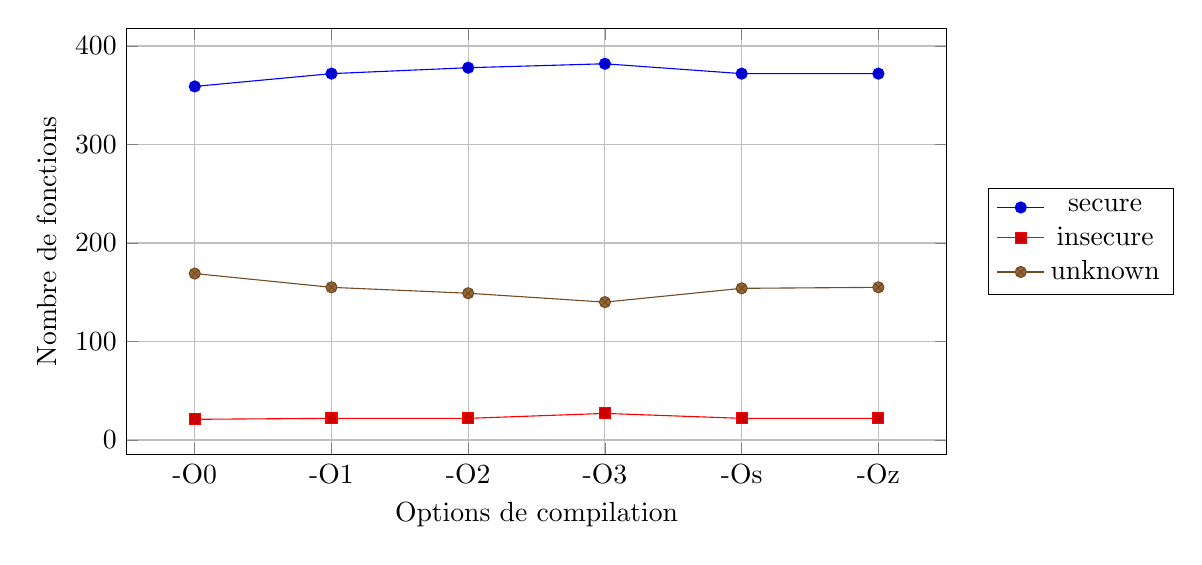
\begin{tikzpicture}
      \begin{axis}[
        xlabel={Options de compilation},
        ylabel={Nombre de fonctions},
        legend style={at={(0.5,-0.15)},anchor=north,legend columns=-1},
        grid=both,
        xtick={0,1,2,3,4,5},
        xticklabels={-O0, -O1, -O2, -O3, -Os, -Oz},
        width=12cm, height=7cm,
        legend style={at={(1.05,0.5)}, anchor=west},
        legend columns=1
      ]

        \addplot coordinates {(0,359) (1,372) (2,378) (3,382) (4,372) (5,372)};
        \addlegendentry{secure}

        \addplot coordinates {(0,21) (1,22) (2,22) (3,27) (4,22) (5,22)};
        \addlegendentry{insecure}

        \addplot coordinates {(0,169) (1,155) (2,149) (3,140) (4,154) (5,155)};
        \addlegendentry{unknown}

      \end{axis}
    \end{tikzpicture}%
  }
  \caption{Graphes des résultats d'Érysichthon en x86\_64}
  \label{fig:graphe_total}
\end{figure}


Les données détaillées peuvent être consultées en annexe \ref{tab:resultats_finaux}. En l'état, l'analyse rapporte entre 139 et 168 fichiers (en fonction des options de compilation, voir la figure \ref{fig:graphe_total}) dont l'analyse n'a pas pu se terminer. Il faudrait observer plus en détails ces fichiers pour connaître les causes précises de ces arrêts. Nous pouvons faire dans un premier temps une analyse haut niveau des raisons probables de ces interruptions. \medbreak

\begin{figure}[!ht]
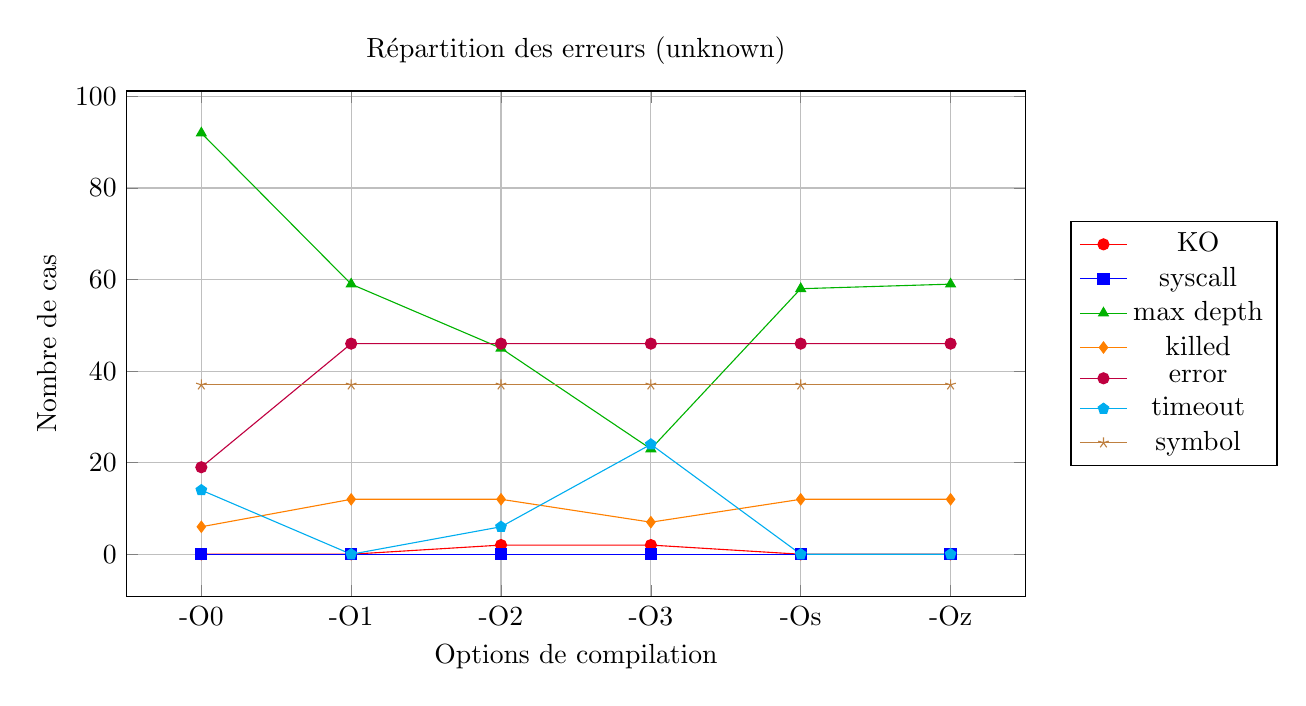
\begin{tikzpicture}
  \begin{axis}[
    title={Répartition des erreurs (unknown)},
    xlabel={Options de compilation},
    ylabel={Nombre de cas},
    grid=both,
    xtick={0,1,2,3,4,5},
    xticklabels={-O0, -O1, -O2, -O3, -Os, -Oz},
    width=13cm, height=8cm,
    legend style={at={(1.05,0.5)}, anchor=west}
  ]

    % KO
    \addplot[color=red, mark=*] coordinates {(0,0) (1,0) (2,2) (3,2) (4,0) (5,0)};
    \addlegendentry{KO}

    % syscall
    \addplot[color=blue, mark=square*] coordinates {(0,0) (1,0) (2,0) (3,0) (4,0) (5,0)};
    \addlegendentry{syscall}

    % max depth
    \addplot[color=green!70!black, mark=triangle*] coordinates {(0,92) (1,59) (2,45) (3,23) (4,58) (5,59)};
    \addlegendentry{max depth}

    % killed
    \addplot[color=orange, mark=diamond*] coordinates {(0,6) (1,12) (2,12) (3,7) (4,12) (5,12)};
    \addlegendentry{killed}

    % error
    \addplot[color=purple, mark=otimes*] coordinates {(0,19) (1,46) (2,46) (3,46) (4,46) (5,46)};
    \addlegendentry{error}

    % timeout
    \addplot[color=cyan, mark=pentagon*] coordinates {(0,14) (1,0) (2,6) (3,24) (4,0) (5,0)};
    \addlegendentry{timeout}

    % symbol
    \addplot[color=brown, mark=star] coordinates {(0,37) (1,37) (2,37) (3,37) (4,37) (5,37)};
    \addlegendentry{symbol}

  \end{axis}
\end{tikzpicture}
  \caption{Graphes détaillant les erreurs interrompant l'analyse Binsec}
  \label{fig:graphe_unknown}
\end{figure}

Le détail des valeurs est rapporté en annexe \ref{table:detail_unknown}.\smallbreak

On peut voir avec cette figure \ref{fig:graphe_unknown} que les erreurs sont dues à :
\begin{enumerate}
  \item[\texttt{max depth}] Arrêt par limitations du nombre d'instruction à analyser, cela permet de réduire la profondeur des branchements conditionnels à explorer et de limiter le risque de parcours infini.
  \item[\texttt{timeout}] Comme le précédent, limitation par le temps. 
  \item[\texttt{killed}] Consommation excessive des ressources, processus interrompu. 
  \item[\texttt{error}] Instruction inconnue de Binsec, il a besoin que le script d'instruction soit corrigé.
  \item[\texttt{symbol}] Comme le précédent, mais peut-être que le fichier de test a besoin d'être modifié.
  \item[\texttt{KO}] Instruction inconnue de Binsec, il a besoin d'être amélioré. 
\end{enumerate}

Chaque erreur préconise un correctif à apporter à Érysichthon. Nous allons détailler les solutions qui nous sont apparus.

\subsection*{Correctifs à implémenter}

Pour résoudre la limitation \texttt{max depth}, nous utiliserons l'outil \texttt{perf}. Cela nous permet de déterminer le nombre d'instructions que contient le binaire. Identifier cette variable nous permet d'exécuter la commande \ref{lst:commande_binsec} précisément.\smallbreak

Concernant l'erreur de type \texttt{timeout}, par défaut une exécution Binsec ne s'interrompt pas, nous avions ajouté ce garde-fou pour forcer l'arrêt de l'analyse de certaines fonctions qui s'étendaient dans le temps. Nos scripts Binsec peuvent être affiné en ciblant précisément les fonctions qui ont besoin de cette limitation. Actuellement, il est sûrement préférable de retirer cette option.\smallbreak

Cela nous amène à l'erreur \texttt{killed}. Ce message n'est pas une erreur provoqué par Binsec mais par un moniteur externe qui vérifie que l'exécution d'Érysichthon ne consomme pas toute la mémoire vive de la machine hôte. Comme présenté au chapitre \ref{chap:erysichtonConception}, l'analyse d'un fichier binaire évolue exponentiellement. Il se trouve que ces fonctions sont comme un sandwich de plus petites fonctions et font exploser la complexité des formules SMT. L'erreur \texttt{max depth} n'est pas déclenché donc il faut sûrement affiner le script Binsec pour ces fonctions.

L'erreur \texttt{symbol} indique une erreur présente dans le scrit Binsec. Cela signifie que le fichier binaire n'a pas le symbole observé par Binsec. Cette erreur est due à un fichier de test produit par Andhrímnir où deux fonctions utilisent des paramètres nommés identiquement. Cette erreur se corrige donc en améliorant le module Andhrímnir.

Pour finir, \texttt{KO} et \texttt{error} sont des erreurs provoqués par Binsec. Dans le premier cas l'instruction binaire lui ait inconnu et dans le second cas il effectue une analyse vers un segment du binaire incompréhensible (fin d'une instruction et début d'une autre ou même une zone sans instruction), il faut donc modifier le script Binsec pour prévenir ce cas de figure.


\subsection*{Sécurité de HACL*}

Revenons sur les résultats présentés sur la figure \ref{fig:graphe_total} et ignorons les fonctions marquées \texttt{unknown}. Les fichiers non sécurisés sont les plus nombreux avec l'option \texttt{-O3} (27) et le moins avec l'option \texttt{-O0} (21). Nous retrouvons le détail des résultats en annexe \ref{tab:resultats_insecure}. Cette expérimentation confirme les travaux de \citeauthor{schneider2024breakingbadcompilersbreak}, dans le sens où augmenter le niveau d'optimisation de compilation augmente le nombre de fonctions qui sont non sécurisées. Nos résultats pourront s'aligner avec l'ajout du compilateur \texttt{LLVM}.\smallbreak 

En revanche, si la question de la sécurité des fonctions identifiées non sécurisées se pose, actuellement la réponse est non. Comme nous analysons toute la bibliothèque HACL*, il est normal que certaines fonctions ne soient pas sécurisées. Elles n'ont pas pour objectif de l'être. Ce sont des fonctions comme \texttt{Hacl\_P256\_\-vali\-date\_public\_key} ou \texttt{Hacl\_P256\_\-ecdsa\_\-verif\_p256\_sha384} qui effectuent des vérifications, des conversions, sur des données publiques. 

Actuellement, dans la liste, aucune fonction indiquée non sécurisée ne demande une réimplémentation et peut être conservée dans la bibliothèque. En première conclusion préliminaire, nous pouvons affirmer qu'il est préférable de ne pas utiliser l'option de compilation \texttt{-O3}.


\vfill
\textit{Ces premiers résultats sont encourageants quant à la méthode employée et laissent de la place à de nombreuses améliorations futures. Une application concrète et exploitable pour l'amélioration de HACL* a été développée et nous permettra d'avoir des garanties formelles sur les binaires utilisables par des utilisateurs de la bibliothèque. Nous allons discuter des actions que nous pouvons réaliser pour perfectionner le travail déjà accompli.}

\backmatter %%%%%%%%%%%%%%%%%%%%%%%%%%%%%%%%%%%%%%%%%%%%%%%%%%%%%%%%%%%%%
\newpage\null\thispagestyle{empty}\newpage
\cleardoublepage
\afterpage{%
    \AddToShipoutPictureBG*{%
\put(9.2cm,20.5cm){
    \fbox{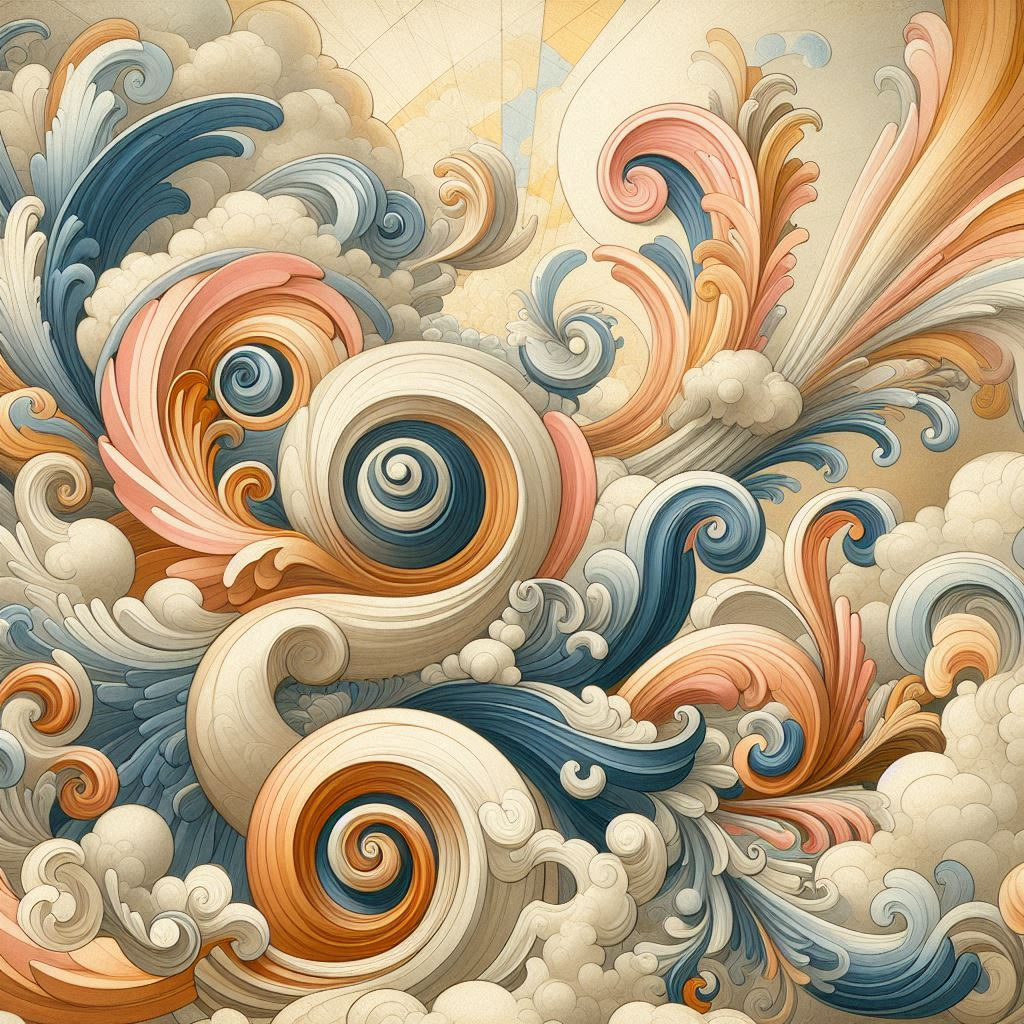
\includegraphics[trim = 12cm 26cm 11cm 0cm, clip, scale = 0.8]{pictures/page_garde.jpeg}}}
    }
    \ClearShipoutPicture%
}
\part{Analyses, projections et conclusion}
\chapter*{Discussion et Ouverture}

\section*{Discussion}

Les résulats obtenues grâce à l'analyse d'Érysichthon ne permettent pas encore de conclure sur la sécurité globale de la bibliothèque Hacl*, il reste encore trop de fonctions non analysées ($\sim 39\%$). En revanche les premiers résultats sont encourageants et montre que l'utilisation des contre-mesures développé au chapitre \ref{chap:constantTimeSolution} est effectivement une bonne pratique. Compléter Érysichthon pour avoir une analyse complète est en tête de liste de la liste des tâche du projet.\medbreak

Actuellement, un seul compilateur a permis de produire ces résultats, il faut absolument étendre l'utilisation à d'autres compilateurs pour pouvoir croiser les résultats et avoir une étude plus complète quant à la sécurité de cette bibliothèque.\smallbreak

Nous savons que les optimisations de compilateur modifient le binaire et peuvent insérer des fuites parce que les modifications changent la structure du programme. Avec cette outil, au lieu d'appeler frontalement \texttt{-O2}, nous pouvons plutôt appeler nominativement les options qui se cachent derrière : \texttt{-falign-functions}, \texttt{-falign-jumps}, \etc. Cette solution permettrait d'identifier les passes de compilateurs qui sont déterminantes pour l'apparition de failles. Il faut en revanche être attentif avec cette solution car \texttt{GCC},utilisé ici, fonctionne différemment de \texttt{LLVM+Clang}. Ce dernier emploie une représentation interne pour effectuer la transformation entre un programme source et un programme binaire.Cette représentation interne évolue entre les différentes étapes de compilations. Cela induit que certaines étapes, même si elle ne nous plaisent pas car elles ajoutent des failles, sont nécessaires pour les suivantes. Nous avons notamment pu croiser ce cas de figures durant notre période de test et à moins d'avoir un code adapté à chaque compilateur, la solution retenu fu de désactiver les optimisations de compilateurs pour le bloc de code concerné.\medbreak

En poursuivant dans cette voie, il nous est aussi possible d'identifier précisément les fonctions qui ont besoins d'être sécurisée et d'adapter leur compilation. Nous pourrions avoir une liste \texttt{sécurisées} qui identifie les fonctions dont la compilation induit trop de dégâts et les autres seraient compilées avec niveau d'optimisation plus élevé. Par exemple, si \textit{A.c} est compilé avec \texttt{-O0}, \textit{A.o} sera généré sans optimisation. De même, si \textit{B.c} est compilé \texttt{-O3}, \textit{B.o} contiendra des fonctions optimisées. Ainsi, dans le binaire final \textit{C.o}, les appels vers une fonction de \textit{A.o} sont des instructions de saut vers le code compilé avec \texttt{-O0}, et les appels vers \textit{B.o} des sauts vers du code compilé avec \texttt{-O3}. Nous obtenons un mélange de fonctions optimisées et non optimisées dans le même exécutable. Cette solution réduira les performances globales et mais préservera un niveau de sécurité plus élevé. Cette solution pave la voie vers une nouvelle étude.\medbreak




\section*{Ouverture}




travaux directement sur le compilateur / support matériel
\addcontentsline{toc}{chapter}{Discussion et Ouverture}
\chapter*{Conclusion}
\addcontentsline{toc}{chapter}{Conclusion}

À travers ce mémoire nous avons vus la mise au point d'Érysichthon, un outil d'analyse automatique de bibliothèque cryptographique. Cette conception a demandé l'implémentation d'un ensemble de module et notamment d'Andhrímnir, un outil de génération de tests. Ce module permet d'avoir au minimum un test par fonctions présentes dans la bibliothèque analysé. Érysichthon est un outil utilisant Binsec, notamment les extensions permettant la vérification formelles des fuites temporelles par l'analyse symbolique non-interférante.\smallbreak

Cette conception c'est réalisé grâce l'étalonnage des réponses à nos questions de recherche. Les travaux de \citeauthor{schneider2024breakingbadcompilersbreak} ont mis en lumière (\textbf{QR1}) que la propagation des garanties de sécurité n'est pas nécessairement conservé lors de la compilation. Vouloir conserver cette propagation demande d'utiliser un compilateur spécialisé et de rajouter des spécifications dans le code source pour préserver le niveau de sécurité attendu. Nous avons aussi pu voir les contraintes inhérente à cette solution, ce qui nous a décidé à explorer d'autres solutions. Celle retenue nous a guidé vers l'étude et l'analyse de binaire après compilation. Cette solution consiste à de vérifier si les éléments de sécurité ont été préservés ou si des fuites sont apparues. Le choix judicieux (\textbf{QR2}) d'utiliser Binsec nous a permis de mettre en place une méthodologie et l'automatisation de l'analyse de binaire à travers un éventail d'architectures et de compilateur. Avec ces briques et de nouveaux protocoles, nous avons pu dresser un cahier des charges (\textbf{QR3}) pour effectuer un changement d'échelle et réussir à concevoir un outil effectuant la vérification de bibliothèque cryptographique.\smallbreak

La première bibliothèque cryptographique vérifié par Érysichthon est HACL*. Cette bibliothèque a la particularité d'être formellement vérifiée et présente des garanties de sécurité à propos du code source de ses fonctions. L'étude \cite{schneider2024breakingbadcompilersbreak} avait mis en lumière des fuites en fonction des compilateurs employés. Nous avons avons reproduis les analyses réalisée et cela nous a permis d'identifier des bogues présent dans Binsec.\smallbreak

Cette étape nous a permis de concevoir des méthodes pour automatiser les analyses manuelles que nous venions de réaliser. La production de protocoles précis et détaillés nous a permis d'accélérer le processus d'implémentation d'Érysichthon et d'effectuer notre première analyse complète de HACL* sur x86\_64 avec \texttt{GCC 12.02}.\smallbreak

Discuter des résulats obtenus nous a permis d'établir une liste de correctifs nécessaire pour avoir une analyse complète d'une bibliothèque cryptographique. Nous avons pu, avec cette analyse de HACL*, concevoir une pré-certification de la sécurité de cette bibliothèque. Nous attestons d'une sécurité de bout en bout, initié formellement dans le code source et conservé au niveau assembleur dans le binaire compilé. 



\addcontentsline{toc}{chapter}{Conclusion}

\nocite{*}
\printbibliography

\mainmatter %%%%%%%%%%%%%%%%%%%%%%%%%%%%%%%%%%%%%%%%%%%%%%%%%%%%%%%%%%%%%%%%%%%%%%%%
\cleardoublepage
\afterpage{%
    \AddToShipoutPictureBG*{%
    \put(4cm,2cm){
        \fbox{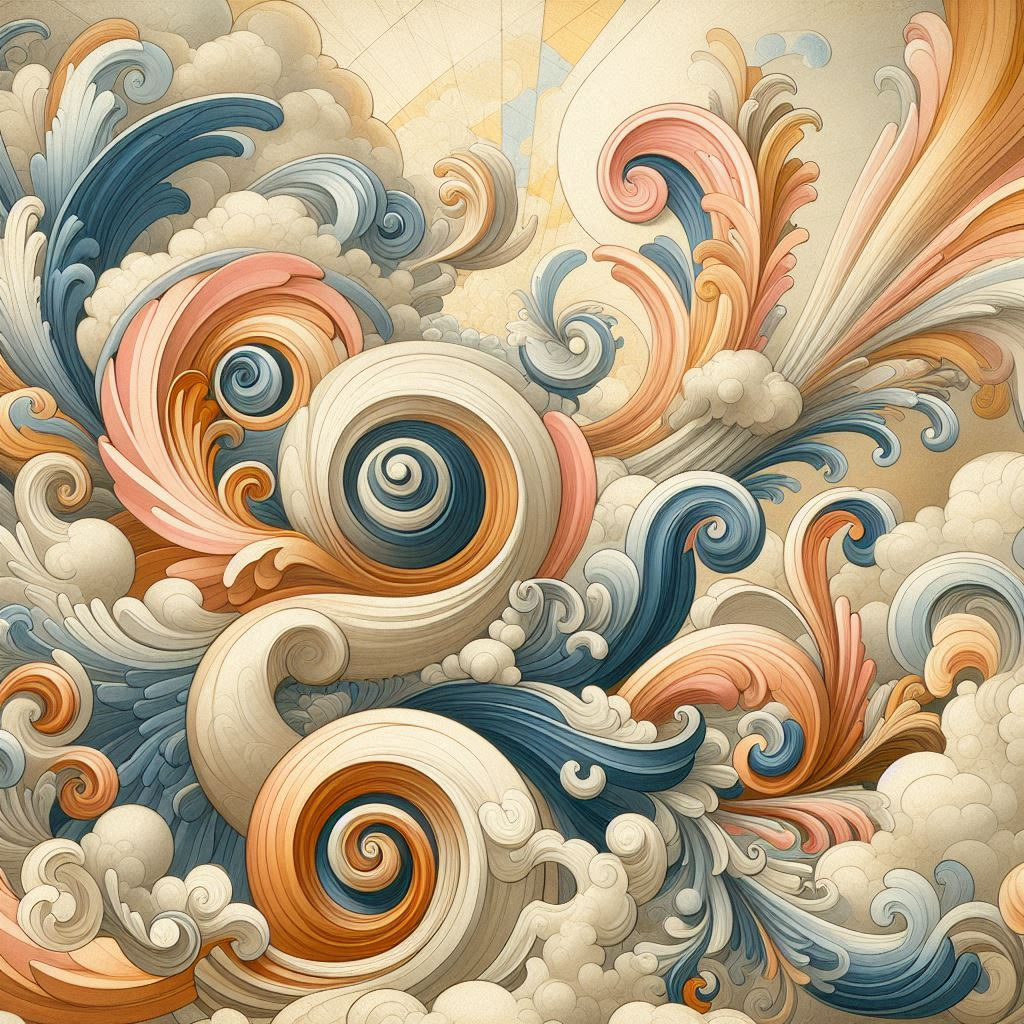
\includegraphics[trim = 7cm 0cm 16cm 24cm, clip, scale = 0.9]{pictures/page_garde.jpeg}}}
    }
    \ClearShipoutPicture%
}
\part*{Annexes}
\addcontentsline{toc}{part}{Annexes}
\appendix
\chapter{Références}

\begin{table}[!ht]
  \caption{Liste des options de compilations et leurs effets (non exhaustive), \url{https://gcc.gnu.org/onlinedocs/gcc/Optimize-Options.html}}
  \label{tab:compile_option}
  \small
  \begin{adjustwidth}{-2.5cm}{-2cm}
  \begin{center}
    \begin{tabular}{ll}
    \hlineB{2}
    \textbf{Option de compilation} & \textbf{Effet} \\
    \rowcolor{lightgray}
    -O0 & Compile le plus vite possible \\
    -O1 / -O & Compile en optimisant la taille et le temps d'exécution \\
    \rowcolor{lightgray}
    -O2 & Comme -O1 mais en plus fort, temps de compilation plus élevé mais exécution plus rapide\\
    -O3 & Comme -O2, avec encore plus d'options, optimisation du binaire\\
    \rowcolor{lightgray}
    -Os & Comme -O2 avec des options en plus, réduction de la taille du binaire au détriment du temps d'exécution  \\
    -Ofast & optimisations de la vitesse de compilation\\
    \rowcolor{lightgray}
    -Oz & optimisation agressive  sur la taille du binaire\\
    \hlineB{2}
    \end{tabular}
  \end{center}
  \end{adjustwidth}
\end{table}

\vfill

\begin{figure}
  \centering
  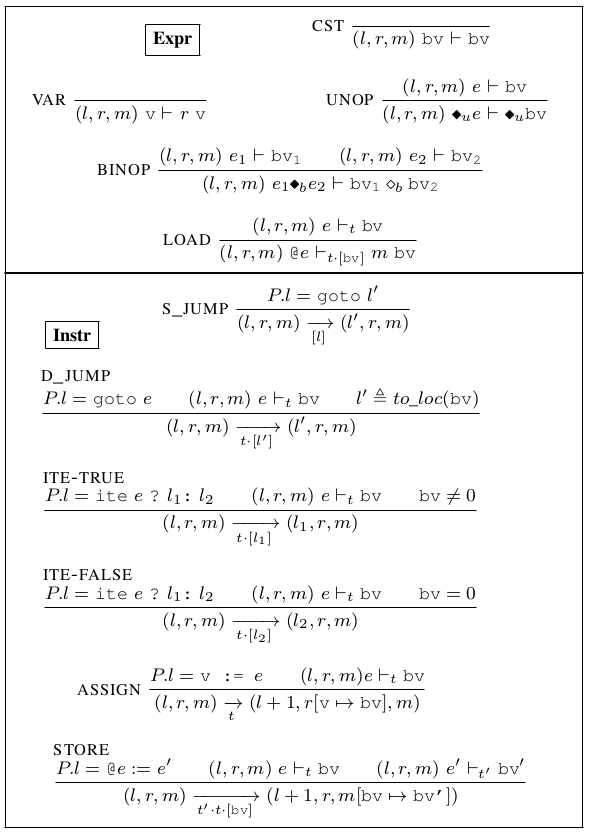
\includegraphics[scale = 0.5]{pictures/instructions_formelles.png}
  \caption{Ensemble d'instructions définis formellement par \cite{binsecRel2019}}
  \label{fig:ensemble_instr_formelles}
\end{figure}


\chapter{Érysichthon, structure, exemples et résultats}

\begin{figure}[!ht]
  \centering
  
  \begin{tikzpicture}[scale= 1.3, transform shape]
    
    % Styles
    \tikzstyle{startstop} = [rectangle, rounded corners, minimum width=2cm, minimum height=1cm, text centered, draw=black, fill=green!30]
    \tikzstyle{process} = [rectangle, minimum width=2cm, minimum height=1cm, text centered, draw=black, fill=orange!30]
    \tikzstyle{arrow} = [thick,->,>=stealth]
    \tikzset{zone1/.style={rectangle, rounded corners, draw=red, dashed, fill=red!10, inner sep=0.3cm}}
    \tikzset{zone2/.style={rectangle, rounded corners, draw=blue, dashed, fill=blue!10, inner sep=0.5cm, text width=3cm}}
    \tikzset{zone3/.style={rectangle, rounded corners, draw=green, dashed, fill=green!10, inner sep=0.3cm}}
    \tikzset{zone4/.style={rectangle, rounded corners, draw=green, dashed, fill=green!30!blue!5, inner sep=0.3cm}}
    
    % Noeuds
    \node (make_test) [startstop] {ANDHRÍMNIR};
    \node (test) [below of = make_test] {Génère les tests};
    \node (test1) [below of=test, xshift=0.5cm, yshift=0.6cm] {\small{test1}};
    \node (test2) [below of=test1, yshift=0.6cm] {\small{test2}};
    \node (test3) [below of=test2, yshift=0.6cm] {\small{test3}};
    \node (test4) [below of=test3, yshift=0.6cm] {\small{test4}};
    \node (dots) [below of=test4, yshift=0.6cm] {\small{$\dots$}};
    
    \foreach \node in {test1, test2, test3, test4, dots} {
      \draw (test.south) |- (\node.west);
      }
      
    \node (start) [startstop, right of=make_test, yshift=2cm, xshift = 4cm] {Érysichthon};
    \node (blanc) [right of=make_test,yshift=-1cm, xshift = 2cm] {};
    \node (compilateur) [below of = start] {Compilateur};
    \node (hacl) [below of = compilateur, xshift=2cm] {Compile Hacl*};
    \node (tests) [below of = hacl, yshift = 0.3cm] {Compile les tests};
    \node (binsec) [below of = tests, xshift=1.8cm] {Exécute Binsec};
    \node (analyse) [below of = binsec, yshift = 0.3cm] {Étude des résultats};
    % Flèches
    \draw [arrow] (compilateur) |- (hacl.west);
    \draw [arrow] (compilateur) |- (tests.west);
    \draw [arrow] (tests) |- (binsec.west);
    \draw [arrow] (tests) |- (analyse.west);

    % Zones
    \begin{scope}[on background layer]
        \node (zone2node) [zone2, fit=(start) (compilateur) (hacl) (tests) (binsec) (analyse) (make_test) (test) (test1) (test2) (test3) (test4) (dots)] {};
        \node (title) [anchor=north west] at (zone2node.north west) {\parbox{3.5cm}{\centering \Huge{\textbf{Érysichthon}}\\\scriptsize{\textit{Panneau de contrôle}}}};
        \node (zone_tests) [zone1, fit=(make_test) (test) (test1) (test2) (test3) (test4) (dots)] {};
        \node (zone_compilation) [zone3, fit=(start) (compilateur) (hacl) (tests) (binsec) (analyse)] {};
        \node (zone_binsec) [zone4, fit=(binsec) (analyse)] {};
    \end{scope}

    % Flèches 2
    
    \draw [arrow, dashed, opacity=0.5] (title) -- (zone_tests);
    \draw [arrow, dashed, opacity=0.5] (title) -- (zone_compilation.west);
    \draw [thick,>=stealth, dashed, opacity=0.4] (title) -- (blanc.north);
    \draw [arrow, dashed, opacity=0.5] (blanc.north) -- (zone_binsec);
    \draw [arrow, dashed, opacity=0.2] (zone_tests.north) -- (zone_compilation.west);
  \end{tikzpicture}
  \caption{Structure d'Érysichthon, schéma du point de vue de l'usager}
  \label{fig:erysichthon_structure}
  \small
  Les flèches grises indiquent tous les éléments actionnables individuellement.
\end{figure}

\newpage
\begin{listing}[!ht]
  \caption{Déclaration de la fonction \textbf{encrypt} dans le fichier d'en-tête Hacl\_AEAD\_\-Chacha20Poly1305\_Simd256.h}
  \label{lst:exemple_header}
  \begin{minted}[
frame=lines,
framesep=2mm,
baselinestretch=1.2,
fontsize=\footnotesize,
linenos
]{c}
/**
Encrypt a message `input` with key `key`.

The arguments `key`, `nonce`, `data`, and `data_len` are same in encryption/decryption.
Note: Encryption and decryption can be executed in-place, i.e.,
`input` and `output` can point to the same memory.

@param output Pointer to `input_len` bytes of memory where the ciphertext is written to.
@param tag Pointer to 16 bytes of memory where the mac is written to.
@param input Pointer to `input_len` bytes of memory where the message is read from.
@param input_len Length of the message.
@param data Pointer to `data_len` bytes of memory where the associated data is read from.
@param data_len Length of the associated data.
@param key Pointer to 32 bytes of memory where the AEAD key is read from.
@param nonce Pointer to 12 bytes of memory where the AEAD nonce is read from.
*/
void
Hacl_AEAD_Chacha20Poly1305_Simd256_encrypt(
  uint8_t *output,
  uint8_t *tag,
  uint8_t *input,
  uint32_t input_len,
  uint8_t *data,
  uint32_t data_len,
  uint8_t *key,
  uint8_t *nonce
);
  \end{minted}
\end{listing}

\vfill
\begin{listing}[!htb]
  \caption{Extrait du fichier Hacl\_AEAD\_Chacha20Poly1305\_Simd256.json}
  \label{lst:exemple_json}
  \begin{minted}[
frame=lines,
framesep=2mm,
baselinestretch=1.2,
fontsize=\footnotesize,
linenos
]{json}
{
"Meta_data":{
    "build" : "13-06-2025",
    "version" : "0.2.0"
}

,"Hacl_AEAD_Chacha20Poly1305_Simd128_encrypt": {
    "*output":"BUF_SIZE"
   ,"*input":"BUF_SIZE"
   ,"input_len":"BUF_SIZE"
   ,"*data":"AAD_SIZE"
   ,"data_len":"AAD_SIZE"
   ,"*key":"KEY_SIZE"
   ,"*nonce":"NONCE_SIZE"
   ,"*tag":"TAG_SIZE"
   ,"BUF_SIZE":16384
   ,"TAG_SIZE":16
   ,"AAD_SIZE":12
   ,"KEY_SIZE":32
   ,"NONCE_SIZE":12
 }
}
  \end{minted}
\end{listing}

\newpage
\begin{listing}[!htb]
  \caption{Code généré du fichier test Hacl\_AEAD\_\-Chacha20\-Poly1305\_Simd256\_\-encrypt.c}
  \label{lst:exemple_complet}
  \begin{minted}[
frame=lines,
framesep=2mm,
baselinestretch=1.2,
fontsize=\footnotesize,
linenos
]{c}
//
// Made by
// ANDHRÍMNIR - 0.5.4
// 12-08-2025
//

#include <stdlib.h>
#include "Hacl_AEAD_Chacha20Poly1305_Simd128.h"

#define BUF_SIZE 16384
#define TAG_SIZE 16
#define AAD_SIZE 12
#define NONCE_SIZE 12
#define KEY_SIZE 32
uint8_t output[BUF_SIZE];
uint8_t tag[TAG_SIZE];
uint8_t input[BUF_SIZE];
uint32_t input_len_encrypt = BUF_SIZE;
uint8_t data[AAD_SIZE];
uint32_t data_len_encrypt = AAD_SIZE;
uint8_t key[KEY_SIZE];
uint8_t nonce[NONCE_SIZE];


int main (int argc, char *argv[]){
Hacl_AEAD_Chacha20Poly1305_Simd128_encrypt(output, tag, input, input_len_encrypt,
 data, data_len_encrypt, key, nonce);
   exit(0);
}
  \end{minted}
\end{listing}

\begin{listing}[!htb]
  \caption{Instruction Binsec générée automatiquement, \\ Hacl\_\-AEAD\_\-Chacha20Poly\-1305\_\-Simd256\_encrypt.ini}
  \label{list:exemple_ini_final}
  \begin{minted}[
frame=lines,
framesep=2mm,
baselinestretch=1.2,
fontsize=\footnotesize,
linenos
]{c}
starting from core

secret global output, input, data, key, nonce, tag
replace opcode 0f 01 d6 by
zf := true
end
replace opcode 0f 05 by
  if rax = 231 then
    print ascii "exit_group"
    print dec rdi
    halt
  end
  print ascii "syscall"
  print dec rax
  assert false
end
halt at <exit>    
  \end{minted}
\end{listing}


\newpage
\begin{table}[!th]
\centering
\begin{adjustwidth}{-20mm}{0mm}
\begin{minipage}{0.48\textwidth}
    \centering
    \begin{tabular}{c|ccc}
        \textbf{Optimisation} & \textbf{Secure} & \textbf{Unknown} & \textbf{Insecure} \\
        \hline
        \rowcolor{blue!5}
        -O0 & 359 & 168 & 21 \\
        -O1 & 372 & 154 & 22 \\
        \rowcolor{blue!5}
        -O2 & 378 & 148 & 22 \\
        -O3 & 382 & 139 & 27 \\
        \rowcolor{blue!5}
        -Os & 372 & 154 & 22 \\
        -Oz & 373 & 153 & 22 \\
    \end{tabular}
    \caption{Résultats d'Érysichthon en x86\_64}
    \label{tab:resultats_finaux}
\end{minipage}%
\hfill
\begin{minipage}{0.48\textwidth}
    \centering
    \begin{tabular}{c|cccccc}
        \textbf{Erreur / Option} & \textbf{-O0} & \textbf{-O1} & \textbf{-O2} & \textbf{-O3} & \textbf{-Os} & \textbf{-Oz} \\
        \hline
        \rowcolor{blue!5}
        KO        & 0  & 0  & 2  & 2  & 0  & 0  \\
        syscall   & 0  & 0  & 0  & 0  & 0  & 0  \\
        \rowcolor{blue!5}
        max depth & 92 & 59 & 45 & 23 & 58 & 59 \\
        killed    & 6  & 12 & 12 & 7  & 12 & 12 \\
        \rowcolor{blue!5}
        error     & 19 & 46 & 46 & 46 & 46 & 46 \\
        timeout   & 14 & 0  & 6  & 24 & 0  & 0  \\
        \rowcolor{blue!5}
        symbole    & 37 & 37 & 37 & 37 & 37 & 37 \\
    \end{tabular}
    \caption{Tableau détaillant les erreurs interrompant l'analyse Binsec}
    \label{table:detail_unknown}
\end{minipage}
\end{adjustwidth}
\end{table}


\raggedleft
\begin{table}[!ht]
  \begin{tabular}{l|cccccc}
    \textbf{Fonctions} & \multicolumn{6}{c}{\textbf{Options concernées}} \\
    \hline
    \rowcolor{blue!5}
    Hacl\_EC\_Ed25519\_point\_eq & O0 & O1 & O2 & O3 & Os & Oz \\
    Hacl\_K256\_ECDSA\_ecdh & O0 & O1 & O2 & O3 & Os & Oz \\
    \rowcolor{blue!5}
    Hacl\_K256\_ECDSA\_ecdsa\_verify\_hashed\_msg & O0 & O1 & O2 & O3 & Os & Oz \\
    Hacl\_K256\_ECDSA\_ecdsa\_verify\_sha256 & O0 & O1 & O2 & O3 & Os & Oz \\
    \rowcolor{blue!5}
    Hacl\_K256\_ECDSA\_is\_public\_key\_valid & O0 & O1 & O2 & O3 & Os & Oz \\
    Hacl\_K256\_ECDSA\_public\_key\_compressed\_from\_raw & O0 & & & & & \\
    \rowcolor{blue!5}
    Hacl\_K256\_ECDSA\_public\_key\_uncompressed\_to\_raw & O0 & O1 & O2 & O3 & Os & Oz \\
    Hacl\_K256\_ECDSA\_secp256k1\_ecdsa\_is\_signature\_normalized & O0 & O1 & O2 & O3 & Os & Oz \\
    \rowcolor{blue!5}
    Hacl\_K256\_ECDSA\_secp256k1\_ecdsa\_signature\_normalize & O0 & O1 & O2 & O3 & Os & Oz \\
    Hacl\_K256\_ECDSA\_secp256k1\_ecdsa\_verify\_hashed\_msg & O0 & O1 & O2 & O3 & Os & Oz \\
    \rowcolor{blue!5}
    Hacl\_K256\_ECDSA\_secp256k1\_ecdsa\_verify\_sha256 & O0 & O1 & O2 & O3 & Os & Oz \\
    Hacl\_NaCl\_crypto\_box\_open\_detached\_afternm & O0 & O1 & O2 & O3 & Os & Oz \\
    \rowcolor{blue!5}
    Hacl\_NaCl\_crypto\_secretbox\_open\_detached & O0 & O1 & O2 & O3 & Os & Oz \\
    Hacl\_P256\_compressed\_to\_raw & O0 & & & & &  \\
    \rowcolor{blue!5}
    Hacl\_P256\_dh\_responder & O0 & O1 & O2 & O3 & Os & Oz \\
    Hacl\_P256\_ecdsa\_verif\_p256\_sha2 & O0 & O1 & O2 & O3 & Os & Oz \\
    \rowcolor{blue!5}
    Hacl\_P256\_ecdsa\_verif\_p256\_sha384 & O0 & O1 & O2 & O3 & Os & Oz \\
    Hacl\_P256\_ecdsa\_verif\_p256\_sha512 & O0 & O1 & O2 & O3 & Os & Oz \\
    \rowcolor{blue!5}
    Hacl\_P256\_ecdsa\_verif\_without\_hash & O0 & O1 & O2 & O3 & Os & Oz \\
    Hacl\_P256\_uncompressed\_to\_raw & O0 & O1 & O2 & O3 & Os & Oz \\
    \rowcolor{blue!5}
    Hacl\_P256\_validate\_public\_key & O0 & O1 & O2 & O3 & Os & Oz \\
    Hacl\_FFDHE\_ffdhe\_shared\_secret\_precomp & & O1 & O2 & O3 & Os & Oz \\
    \rowcolor{blue!5}
    Hacl\_K256\_ECDSA\_secp256k1\_ecdsa\_sign\_hashed\_msg & & O1 & O2 & O3 & Os & Oz \\
    Hacl\_K256\_ECDSA\_secp256k1\_ecdsa\_sign\_sha256 & & O1 & O2 & O3 & Os & Oz \\
    \rowcolor{blue!5}
    Hacl\_NaCl\_crypto\_box\_beforenm & & & & O3 & &  \\
    Hacl\_NaCl\_crypto\_box\_detached & & & & O3 & &  \\
    \rowcolor{blue!5}
    Hacl\_NaCl\_crypto\_box\_easy& & & & O3 & &  \\
    Hacl\_NaCl\_crypto\_box\_open\_detached & & & & O3 & & \\
    \rowcolor{blue!5}
    Hacl\_NaCl\_crypto\_box\_open\_easy& & & & O3 & &  \\
  \end{tabular}
  \caption{Détails des fonctions non sécurisées en fonction des optimisations entrées, éxecution d'Érysichthon en x86\_64}
  \label{tab:resultats_insecure}
\end{table}


\end{document}
